\documentclass{llncs}
\usepackage{times}
\usepackage{csp}
\usepackage[boxruled,linesnumbered]{algorithm2e}
\usepackage{algpseudocode}
\usepackage{float, graphicx, epstopdf, lipsum, fancyhdr}
\usepackage{wrapfig}
\usepackage{subfigure}
\begin{document}

\title{Loop Invariant Generation through Active Learning}
\author{
Jiaying Li, Li Li, Le Guang Loc, Jun Sun\\
\institute{
Singapore University of Technology and Design \\
\email{jiaying\_li@mymail.sutd.edu.sg\\ \{li\_li,guangloc\_le,sunjun\}@sutd.edu.sg}}
}

\maketitle

\begin{abstract}
	Loop invariant generation is one of the fundamental problems in program analysis and verification. 
    In this work, we propose an automatic generation method for inductive loop invariants 
    through iterations of runtime sampling, machine learning and constraint solving. 
    In each iteration, our method first collects real data at runtime based on selective sampling. 
    Then, based on their satisfaction of the assumptions and assertions in the program, 
    our method uses support vector machine to learn a loop invariant candidate, 
    i.e., a conjunction of linear and polynomial constraints. 
    Finally, if the candidate can be verified as the inductive loop invariant of the program, 
    our method returns it directly and ends the generation process. 
    Otherwise, the counter-example is used to refine the data sampling in the next iteration. 
    The experiment evaluation shows that our method can be used to learn loop invariants 
    effectively and automatically that cannot be learned by other loop invariant generation tools. 
\end{abstract}

%!TEX root = paper.tex

\section{Introduction} % (fold)
\label{sec:introduction}

Automatic loop invariant generation is fundamental for program analysis. A loop invariant can be useful for software verification, compiler optimization, program understanding, etc. In the following, we first define the loop invariant generation problem and then briefly describe existing approaches and then our proposal. For simplicity, we assume that we are given a Hoare triple in the following form. 
%\[
%    P = \{ \mathit{Pre} \} \mathit{while}(\mathit{Cond}) \{ \mathit{Body} \} \{ \mathit{Post} \}
%\]
\begin{align*}
&\{\mathit{Pre}\} & & /\star\text{\emph{Assumption}}\star/ \\
&\mathit{while} (\mathit{Cond}) \{ \mathit{Body} \} && /\star\text{\emph{Loop Body}}\star/\\
&\{\mathit{Post}\} & & /\star\text{\emph{Assertion}}\star/
\end{align*}
Assume that $V = \{x_1{,} x_2{,} \cdots{,} x_n\}$ is a finite set of program variables which are relevant to the loop body. $\mathit{Pre}$, $\mathit{Cond}$ and $\mathit{Post}$ are predicates constituted by variables in $V$.

\begin{align*}
&\{\mathit{Pre}\} & & \emph{Pre} \Rightarrow \emph{Inv} \\
&\mathit{while} (\mathit{Cond}) \{ \mathit{Body} \} && \{\emph{Inv} \wedge \emph{Cond}\} \emph{Body} \{\emph{Inv}\}\\\
&\{\mathit{Post}\} & & \emph{Inv} \wedge \neg \emph{Cond} \Rightarrow \emph{Post}
\end{align*}
%In practice, the pre-condition $\mathit{Pre}$ is often described by
%the specification documents and checking conditions of the program inputs,
%and the post-condition $\mathit{Post}$ is usually specified
%by assertions and exceptions leading to an error state in the program.
Let $s = \{ x_1 \mapsto v_1, \ldots, x_n \mapsto v_n \}$ be a valuation of $V$. Let $\phi$ be a predicate constituted by variables in $V$. We write $s \models \phi$ to denote that $\phi$ is evaluated to $\mathit{true}$ given the program state $s$. Otherwise, we write $s \not \models \phi$. 
$\mathit{Body}$ is an imperative program which updates the valuation of $V$. For simplicity, we assume that it is a deterministic function on valuations of variables $V$, and write $\mathit{Body}(s)$ to denote the valuation of $V$ after executing $\mathit{Body}$ given the initial variable valuation $s$. For convenience, $\mathit{Body}^i(s)$ where $i \geq 0$ is defined as follows: $\mathit{Body}^0(s) = s$ and $\mathit{Body}^{i+1}(s) = \mathit{Body}(\mathit{Body}^i(s))$.
%the evaluation function of the program variables $x_1, \ldots, x_n$
%and $\mathit{Body}(s)$ stand for their new evaluation after the execution of $\mathit{Body}$,
%the above program means that (1) $\mathit{Pre}$ is the assumption to the initial value of $s$;
%(2) if the $\mathit{Cond}$ is satisfied by $s$ at an iteration,
%$\mathit{Body}$ will be executed and $s$ will be updated to $\mathit{body}(s)$;
%(3) if the $\mathit{Cond}$ is unsatisfied by $s$ at an iteration,
%the while-loop ends and $s$ should satisfy $\mathit{Post}$.

In order to prove the Hoare triple, we would like to find a loop invariant $\mathit{Inv}$ which satisfies the following three conditions.
\begin{align}
    &s \models \mathit{Pre}
        &&\Longrightarrow & s &\models \mathit{Inv} \label{inv:pre} \\
    &s \models \mathit{Inv} \wedge \mathit{Cond}
        &&\Longrightarrow & \mathit{Body}(s) &\models \mathit{Inv} \label{inv:loop} \\
    &s \models \mathit{Inv} \wedge \neg \mathit{Cond}
        &&\Longrightarrow & s &\models \mathit{Post} \label{inv:post}
\end{align}
Alternatively, we would like to find a valuation $s$ such that $s \models \mathit{Pre}$ and executing the loop until it terminates results in a valuation $s'$ such that $s' \not \models \mathit{Post}$.
The problem is thus either to prove the Hoare triple (by identifying an $\mathit{Inv}$ satisfying the three conditions) or to disprove it (by finding a valuation $s$ as described above). For simplicity, we further assume that the loop body always terminates and refer the readers to~\cite{Domagoj:FAC:2013,LeQC:PLDI:15,Hong:ASE:2015} %%\cite{acmcomm}
for extensive research on proving loop termination.

Many approaches have been proposed for the invariant generation.
For example, there are proposals based on abstraction interpretation~\cite{cousot1978automatic,mine2006octagon,cousot1979systematic,karr1976affine,vincent2009subpolyhedra}, counterexample guided abstraction refinement~\cite{henzinger2003software,thomas2001slam,edmund2003counterexample}, interpolation~\cite{kenneth2010lazy,thomas2004abstractions,kenneth2003interpolation,Kenneth2006lazy} and constraint solving and inference~\cite{ashutosh2009invgen,michael2003linear,sumit2009constraint}.
Recently, the authors of~\cite{sharma2012interpolants,sharma2013verification,DBLP:conf/esop/0001GHALN13,sharma2014invariant} proposed to automatically generate loop invariants based on random searching~\cite{sharma2014invariant} as well as machine learning~\cite{sharma2012interpolants}.
Their approaches start with randomly generating valuations of $V$ (a.k.a.~the samples) and categorize them into different groups, e.g., one containing those satisfying the loop invariant $\mathit{Inv}$ (if there is any) and another containing those not. Machine learning techniques are then used to generalize them in a certain form to obtain candidate loop invariants.
%For instance, classification algorithms like Support Vector Machines (SVM) ~\cite{sharma2012interpolants} can be used to generate classifiers as candidate invariants.
The candidates are then checked using program verification techniques (like symbolic execution~\cite{symbolic}) to see whether they satisfy the three conditions. If a certain condition is violated, we obtain counterexamples in the form of variable valuations.
For instance, given a candidate $\phi$, if condition (1) is violated, a valuation $s$ satisfying $s {\models} Pre {\land} s {\not \models} \phi$ is generated, which proves that $\phi$ is not an invariant.
With this new sample, we can apply the classification algorithm again to obtain a new candidate invariant. The learn-and-check process is iteratively repeated until an invariant satisfying all three conditions is identified or a valuation disproving the Hoare triple is found.

One problem with the above approach is that its effectiveness is often limited by the samples which are generated either randomly. In order to learn the right invariant through classification, often a large number of samples are necessary. Furthermore, often we must have those samples right by the boundary between variable valuations which satisfy the actual invariant and those which do not, so that classification techniques would identify the right invariant. Obtaining those samples through random sampling is often hard. As a result, many iterations of learn-and-check are necessary before the candidate invariant converges to the right one. Another problem is that the loop invariants obtained through existing learn-and-check approaches~\cite{sharma2012interpolants,sharma2013verification,DBLP:conf/esop/0001GHALN13,sharma2014invariant} are limited, e.g., linear inequalities or their conjunctions in~\cite{sharma2012interpolants}, and equalities in~\cite{DBLP:conf/esop/0001GHALN13}.

In this work, we propose a framework for loop invariant generation following the same learn-and-check approach. %We improve existing approaches in two aspects. First, by adopting active learning techniques, we improve the quality of the candidate invariants prior to verifying them, in every iteration of learn-and-check. As a result, we can reduce the number of learn-and-check iterations significantly. Second, by supporting an extensible framework, we can easily integrate different classification techniques (e.g., SVM with kernel methods~\cite{}) as well as the corresponding active learning techniques so that we can learn a large class of invariants. %We have developed a prototype implementation of our method and applied to benchmark programs including those from the software verification competition. The results show that our method often reduces the number of guess-and-check iterations as well as is able to learning more loop invariants than existing approaches.
%In the following, we define our problem and briefly illustrate how our approach works.
Compared to the existing approaches, we make the following contributions. Firstly, we propose an active learning technique to (partially) overcome the limitation of random sampling. That is, the active learning technique allows us to automatically generate samples which are important in improving the quality of the candidate invariants so that we can improve the candidates prior to verifying them during every learn-and-check iteration. As a result, we can reduce the number of learn-and-check iterations significantly, or even completely in some cases.
%    for automatic invariant inference based on machine learning.
%    Since the samples are chosen for clear purpose
%    to refine the invariant candidate in the \emph{data collection} stage,
%    the invariant converges efficiently.
%    Furthermore, because the counter-examples generated in the \emph{invariant verification} stage
%    give very accurate information to amend the invariant candidate,
%    they become a useful supplementary to overcome the weakness of machine learning
%    and fine-tune the invariant candidate.
Secondly, our framework is designed to be extensible for learning different invariants. For instance, we show that we can easily extend our framework to learn candidate invariants in the form of polynomial inequalities or their conjunctions.
Lastly, we implement our framework as a tool called \textsc{Zilu}~\cite{zilu:repo}
    and compare it with Interproc~\cite{jeannet2010interproc}, %% other
an available state-of-the-art invariant inference tool.
%%    i.e., 
    %CPAChecker~\cite{beyer2011cpachecker} and 
 %%   Interproc~\cite{jeannet2010interproc}.
%    Our experiment results show that
%    we are the only tool that can work with polynomial invariant inference.
%    Notice that the polynomial invariant inference works in our framework
%    naturally with very light additional programming.
    % Based on the design of different approaches,
    % we also claim that our framework have better extensibility comparing with their method.
    \textsc{Zilu} is built upon existing tools (e.g., GNU Scientific Library ($\mathit{GSL}$)~\cite{gough2009gnu} for active learning,
    $\mathit{LibSVM}$~\cite{chang2011libsvm} for $\mathit{SVM}$ classification,
    revised $\mathit{KLEE}$~\cite{cadar2008klee} for symbolic execution~\cite{king1976symbolic,symbolic}, and Z3~\cite{de2008z3} for verification) and 
    can be used as a language/platform independent tool to verify programs.

\paragraph{Organization} The remainders of the paper are organized as follows. Section~\ref{sec:overview} presents an overview of our approach using an illustrative example. Section~\ref{sec:sampling} and~\ref{sec:learning} then presents details on two main steps in our framework: data collection and active learning. Section~\ref{sec:evaluations} discusses our prototype implementation and evaluates its effectiveness using a set of benchmark programs. Section~\ref{sec:related} reviews related work and concludes.

\section{Overview through an Example} \label{sec:overview}
In our framework, loop invariant generation is an iterative process of \emph{data collection}, \emph{active learning} and \emph{candidate verification}. The overall workflow is shown in the Figure~\ref{fig:overview}. In the following, we use a simple example to illustrate how our approach works.

\begin{figure}[t]
    \centering
    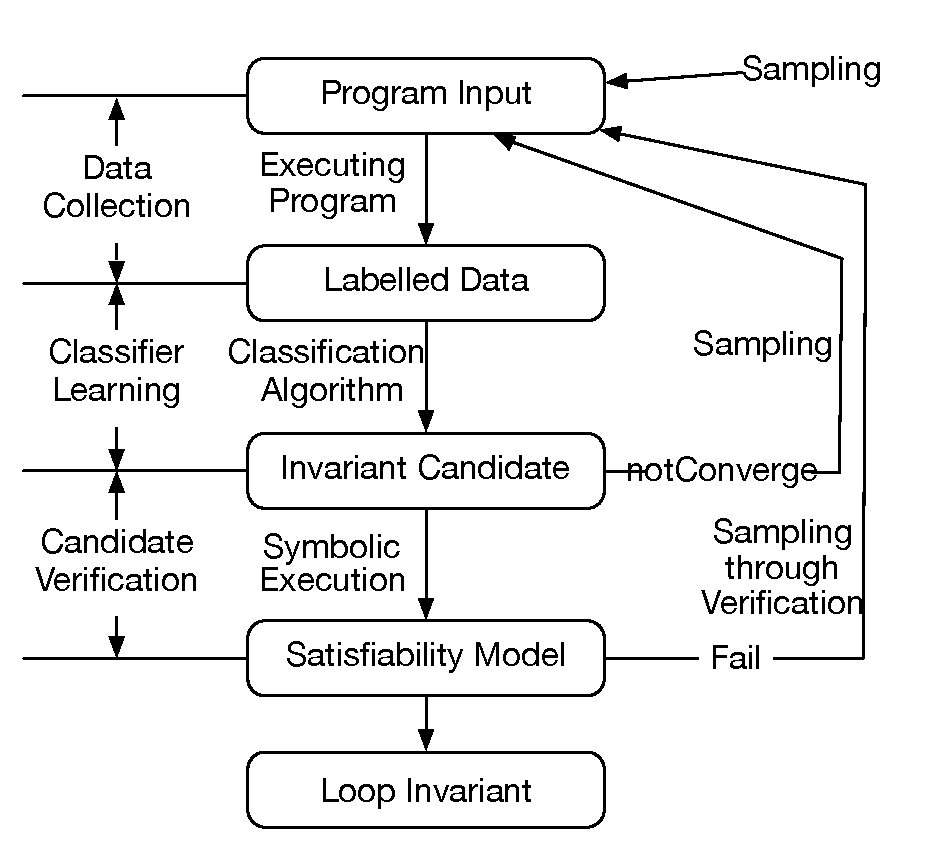
\includegraphics[scale=0.45]{figures/overview.pdf}
    \caption{Loop Invariant Inference Framework Overview}
    \label{fig:overview}
\end{figure}

\begin{figure}[t]
\begin{subfigure}{0.5\textwidth}
    \raggedright
    \vspace{0.5cm}
%% {\scriptsize\begin{verbatim}
%% void P(int x, int y) {
%%     assume(x < y);
%%     while (x < y) {
%%         if (x < 0) x = x + 7;
%%         else x = x + 10;

%%         if (y < 0) y = y - 10;
%%         else y = y + 3;
%%     }
%%     assert(x >= y
%%         && x <= y + 16);
%% }
%% \end{verbatim}}
\vspace{-0.2cm} \[
 \begin{array}{ll}
1 & \code{void~P(int ~x{,} ~int~y)\{} \\
2 & \code{~~~ assume(x~{<}~y);}  \\
3 & \code{~~~ while(x~{<}~y)\{}  \\
4 & \code{~~~ \quad if~(x~{<}~0)~x~{=}~x~{+}~7;}  \\
5 & \code{~~~ \quad else~ x~{=}~x~{+}~10;}\\
6 & \code{~~~ \quad if~(y~{<}~0)~y~{=}~y~{-}~10;} \\
7 & \code{~~~ \quad else~ y~{=}~y~{+}~3;}\\
8 & \code{~~~\}} \\
9 & \code{~~~assert(x~{\geq}~y}\\
10 & \code{~~~\quad \&\&~x~{\leq}~y~{+}~16);}\\
11  & \}
\end{array}
\]
    \vspace{-0.2cm}
    \caption{A sample program}
    \label{fig:running:example:program}
\end{subfigure}%
\begin{subfigure}{.5\textwidth}
      \centering
      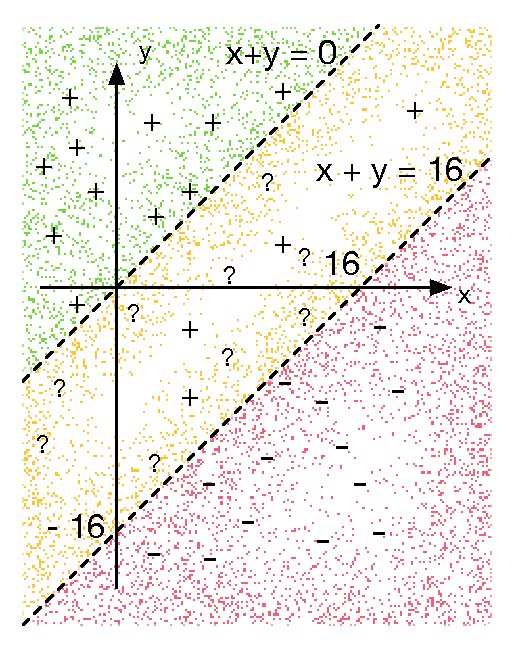
\includegraphics[scale=0.42]{figures/running-sampling.pdf}
      \caption{Sampling}
      \label{fig:running:example:sampling}
\end{subfigure}
\caption{A running example}
\label{fig:running:example}
\end{figure}
%%%sunjun: the two lines should x - y = 0 and x - y = 16.


\begin{example}
An example Hoare triple is shown in Figure~\ref{fig:running:example:program} (where an \code{assume} statement captures the precondition and an \code{assert} statement captures the postcondition). 
The set of variables $V$ contains two integer-type ones: $x$ and $y$. 
For simplicity, we interpret integers in the programs as mathematical integers (i.e., they do not overflow). 
The precondition $\mathit{Pre}$ is $\mathit{x < y}$, which is the same as the loop condition $\mathit{Cond}$.
During each loop iteration, $x$ is increased by $7$ if it is negative (line 4); otherwise, it is increased by $10$ (line 5). 
$y$ is decreased by $10$ if it is negative (line 6); 
otherwise, it is increased by $3$ (line 7). 
The postcondition $\mathit{Post}$ is $\mathit{y \le x \le y + 16}$. 
It is easy to check that the Hoare triple can be proven using a loop invariant $\mathit{Inv}$: $\mathit{x \le y + 16}$. 
In the following, we show how our framework works to learn this loop invariant.
\end{example}
We start with \emph{data collection}. Given the Hoare triple, we first  generate a set of valuations of $V$ randomly. 
% For instance, we can adopt a constraint solver to generate random valuations which satisfy or fail $\mathit{Pre}$ as random samples.
%For each sample $s_0$ (i.e., a variable valuation) $\in V$, 
Then we execute the loop program with $s_0 \in V$ as the initial evaluation and record an evaluation sequence $\{s_0, s_1, s_2, \cdots, s_i, \cdots, s_n\}$ after each iteration of the loop. 
%We donate $s_0$ as the initial evaluation of $s_i$, and $s_n$ as the last evaluation of $s_i$.
%We write $s_i$ as the state after the $i_{th}$ iteration of the loop. %, ~ {0<=i<=n}$
%as a trace $\langle s_0, s_1, \ldots, s_n \rangle$ where $s_n \not \models Cond$. Let $T$ denote the set of traces. We write $s \Rightarrow_T s'$ to denote that there exists a trace $\langle s_0, s_1, \cdots, s, \cdots, s', \cdots, s_n \rangle \in T$.
All the variable valuations $s_i~(0 \leq i \leq n)$ in such an evaluation sequence are divided into the following four sets according to whether $s_0$ satisfies $\mathit{Pre}$ and $s_n$ satisfies $\mathit{Post}$.
Let $\mathit{Inv}$ be any invariant which satisfies condition (1), (2) and (3). 
\begin{itemize}
    \item Set $\mathit{CE}$ contains all the valuations $s_i$ in an evaluation sequence where $\mathit{s_0 \models \mathit{Pre}}$ but $\mathit{s_n \not\models \mathit{Post}}$. We remark that anytime a valuation in $\mathit{CE}$ is identified, a counterexample is found and the Hoare triple is falsified.
    \item Set $\mathit{Positive}$ contains all the valuations $s_i$ in an evaluation where $\mathit{s_0 \models \mathit{Pre}}$ and $\mathit{s_n \models \mathit{Post}}$. In Section~\ref{sec:sampling} we prove that any valuation in $\mathit{Positive}$ must satisfy $\mathit{Inv}$, if $\mathit{Inv}$ exists.
    \item Set $\mathit{Negative}$ contains all the valuations $s_i$ in an evaluation where $\mathit{s_0 \not\models \mathit{Pre}}$ and $\mathit{s_n \not\models \mathit{Post}}$. In Section~\ref{sec:sampling} we prove that any valuation in $\mathit{Negative}$ must fail $\mathit{Inv}$, if $\mathit{Inv}$ exists.
    \item Set $\mathit{NP}$ contains all the valuations which have not appeared in the above three sets. The satisfaction of these valuations to $\mathit{Inv}$ can not be decided according to the current knowledge. So they may or may not satisfy $\mathit{Inv}$.
\end{itemize}
%\begin{itemize}
%    \item Set $\mathit{CE}$ contains the set of valuations which satisfy the precondition and violate the postcondition afterwards. We remark that anytime a valuation in $\mathit{CE}$ is identified, a counterexample is found and the Hoare triple is falsified.
%    \item Set $\mathit{Positive}$ contains the set of valuations which must satisfy $\mathit{Inv}$.
%    \item Set $\mathit{Negative}$ contains the set of valuations which must fail $\mathit{Inv}$.
%    \item Set $\mathit{NP}$ contains the set of valuations which may or may not satisfy $\mathit{Inv}$.
%\end{itemize}
%The exact definition of these sets is in Section~\ref{sec:sampling}.
% Otherwise, because $\mathit{Inv}$ must satisfy (1),(2) and (3), we know that $P_T \subseteq Inv$ and $N_T \cap Inv = \emptyset$. The program states in $NP_T$ may or not may be in $\mathit{Inv}$. If we know that a program state $s \in NP_T$ is in $\mathit{Inv}$, $Body^*(s) \subseteq Inv$.
%
%Each trace is then associated with a pair of boolean labels $(SatPre, SatPost)$
%
%    All of the evaluations in the above trace (referred by its initial evaluation $s_0$)
%    are labelled based on a pair of boolean values
%    $(s_0 \models \mathit{Pre}, s_n \models \mathit{Post})$\footnote{
%        $(\mathit{true}, \mathit{true}) \rightarrow +$,
%        $(\mathit{false}, \mathit{false}) \rightarrow -$
%        and $(\mathit{false}, \mathit{true}) \rightarrow ?$}.
\begin{example}
We illustrate these four sets using the example shown in Figure~\ref{fig:running:example}. Since the Hoare triple is valid, set $\mathit{CE}$ for this example is empty. 
Assume that the following three valuations are randomly sampled initially in our running example: $\mathit{\{x \mapsto 1, y \mapsto 2\}}$, $\mathit{\{x \mapsto 10, y \mapsto 1\}}$ and $\mathit{\{x \mapsto 100, y \mapsto 0\}}$. 
Three sequences of valuations are generated accordingly: $\mathit{\langle \{x \mapsto 1, y \mapsto 2\}, \{x \mapsto 11, y \mapsto 5\} \rangle}$, $\mathit{\langle \{x \mapsto 10, y \mapsto 1\} \rangle}$ and $\mathit{\langle \{x \mapsto 100, y \mapsto 0\} \rangle}$. 
Note that the loop is not executed for the latter two cases. 
As a result, set $\mathit{Negative}$ contains $\mathit{\{x \mapsto 100, y \mapsto 0\}}$; 
set $\mathit{Positive}$ contains $\mathit{\{x \mapsto 1, y \mapsto 2\}}$ and $\mathit{\{x \mapsto 11, y \mapsto 5\}}$; 
and $\mathit{NP}$ contains $\mathit{\{x \mapsto 10, y \mapsto 1\}}$.
\end{example}
Next, we move on to \emph{active learning} to generate candidate invariants based on $\mathit{Positive}$, $\mathit{Negative}$ and $\mathit{NP}$. 
Intuitively, since we know that valuations in $\mathit{Positive}$ must satisfy $\mathit{Inv}$ and valuations in $\mathit{Negative}$ must not satisfy $\mathit{Inv}$, 
a predicate separating the two sets (a.k.a.~a classifier) could be a candidate for $\mathit{Inv}$.
%Formally, a classifier between two sets $P$ and $N$ is a predicate $\phi$ such that $s \models \phi$ for all $s \in P$ and $s \not \models \phi$ for all $s \in N$.
For instance, Figure~\ref{fig:running:example:sampling} shows where the set of valuations 
in $\mathit{Positive}$, $\mathit{Negative}$ and $\mathit{NP}$ locate geographically in a 2-D plane for our running example. %if we consider only the variable valuation before the loop. 
In particular, valuations in $\mathit{Positive}$ are labeled with $+$; % and color green; 
valuations in $\mathit{Negative}$ are labeled with $-$; % and color red; 
and valuations in $\mathit{NP}$ are labeled with ?. % and color yellow. 
%Note that if variable valuations after some iterations of the loop are considered, some of the valuations categorized as $NP$ in Figure~\ref{fig:running:example:sampling} may be in $Positive$ instead as we show in Section~\ref{sec:sampling}.
%, such as $\{x \mapsto 11, y \mapsto 5\} \rangle$.
And there are three areas: a pure positive area with color green, a pure negative area with color red, and a mixed area with color yellow.
The existence of a mixed area is caused by our labeling method which depends much on the observed program valuation sequences.
For example, $\mathit{\{x \mapsto 11, y \mapsto 5\}}$, labeled as `+' in Fig.~\ref{fig:running:example:sampling}, 
could also be labeled as `?' if it only appears in an one execution valuation sequence $\mathit{\langle \{x \mapsto 11, y \mapsto 5\} \rangle}$.
It can be observed the classifier separating $\mathit{Negative}$ from the rest (i.e., $\mathit{x - y \leq 16}$) 
is the loop invariant we are searching for. 
%If we do execute the program with $\{x \mapsto 11, y \mapsto 5\} \rangle$

In order to automatically generate candidate invariants, we apply existing classification techniques to generate classifiers. 
There are however two issues to be solved. The first issue is, with the limited samples in $\mathit{Positive}$ and $\mathit{Negative}$, 
it is unlikely that we can obtain an ``accurate'' classifier. 
For instance, given the above-mentioned set $\mathit{Positive}$ and $\mathit{Negative}$, 
a classifier identified using classification techniques like $\mathit{SVM}$ could be: $\mathit{3x-10y \leq 152}$. %$x+y \leq 50$. 
Although this classifier perfectly separates the current valuations in $\mathit{Positive}$ from $\mathit{Negative}$. 
it is far from our wanted loop invariant and is clearly the result of having limited samples. 
Researchers in the machine learning community have studied extensively on how to overcome the problem of limited samples and one of the remedies is active learning~\cite{DBLP:series/synthesis/2012Settles}. 
Active learning is a semi-supervised machine learning in which a learning algorithm is able to interactively ask for samples which are important in improving a given classifier. 
For instance, active learning for $\mathit{SVM}$ works by repeatedly generating samples on (or nearby) the current classification boundary, adding them into $\mathit{Positive}$ and $\mathit{Negative}$ accordingly and applying $\mathit{SVM}$ to generate new classifiers. 
This process is repeated until the classifier converges. It has been shown that active learning effectively learns an accurate function with fewer samples~\cite{DBLP:conf/icml/SchohnC00}.

\begin{example}
In the above example, given the current classifier $\mathit{3x-10y \leq 152}$, we apply active learning for $\mathit{SVM}$ 
and generate new valuations $\mathit{\{x \mapsto 7, y \mapsto -13\}}$ and $\mathit{\{x \mapsto 14, y \mapsto -11\}}$ %$\{x \mapsto 44, y \mapsto -2\}$ 
by solving the equation $\mathit{3x-10y = 152}$. % (and using an existing $x$ values to figure out the corresponding $y$ value and vice versa). 
Next, we execute the program with these variable valuations, obtain the variable valuation sequences, and add them into $\mathit{CE}$, $\mathit{Positive}$, $\mathit{Negative}$ or $\mathit{NP}$ accordingly. 
With these new samples, a new classifier is then learnt by applying classification algorithms.
\end{example}
The other issue is: how do we handle those valuations in $\mathit{NP}$, which may or may not satisfy $\mathit{Inv}$? 
If we simply ignore them, there may be a gap between $\mathit{Positive}$ and $\mathit{Negative}$ 
and as a result, the learnt classifier may not converge to the invariant we want, even with the help of active learning. 
This is illustrated in Figure~\ref{fig:running:example:sampling}, where $\mathit{NP}$ happens to be located in between $\mathit{Positive}$ and $\mathit{Negative}$. 
Without considering the samples in $\mathit{NP}$, multiple classifiers located in the $\mathit{NP}$ region (e.g., $\mathit{x - y \leq 10}$, or $\mathit{x - y \leq 15}$) may be learnt to perfectly classify $\mathit{Positive}$ and $\mathit{Negative}$. 
Identifying more samples in $\mathit{Positive}$ or $\mathit{Negative}$ may not help to improve the classifier either. 
To overcome the problem, in addition to learn a classifier separating $\mathit{Positive}$ and $\mathit{Negative}$, we learn two additional candidate invariants making use of $\mathit{NP}$: 
one separating $\mathit{Positive}$ from $\mathit{Negative}$ and $\mathit{NP}$ (i.e., assuming valuations in $\mathit{NP}$ fail $\mathit{Inv}$); 
and the other separating $\mathit{Negative}$ from $\mathit{Positive}$ and $\mathit{NP}$ (i.e., assuming valuations in $\mathit{NP}$ satisfy $\mathit{Inv}$). 
We remark that active learning is applied to all three candidates until they converge. 
In our example, if we restrict our learning classifier to linear inequation, 
the classifier separating $\mathit{Positive}$ from $\mathit{Negative}$ and $\mathit{NP}$ would be $\textsc{null}$ (no such a linear classifier); % $\emptyset$, %converge to $\varnothing$ %$\mathit{NULL}$; %x - y \leq 0$; 
and the classifier separating $\mathit{Negative}$ from $\mathit{Positive}$ and $\mathit{NP}$ would converge to $\mathit{x - y \leq 16}$.

After all three candidate invariants converge, we move on to \emph{candidate verification}. 
We check whether any of the candidate invariants satisfies condition (1), (2) and (3). 
In particular, for each candidate invariant $\phi$, we check whether any of the following formula is satisfiable or not using an $\mathit{SMT}$solver~\cite{barrett2009satisfiability,de2008z3}.
\begin{align}
    & \mathit{Pre} \land \neg \phi \label{check:inv:pre} \\
    %% & (s \models \phi \land \mathit{Cond}) \land (\mathit{Body}(s) \not \models \phi) \label{check:inv:loop} \\
     & sp(\phi \land \mathit{Cond}, \mathit{Body}) \land \neg \phi \label{check:inv:loop} \\
    & \phi \land \neg \mathit{Cond} \land \neg \mathit{Post} \label{check:inv:post}
\end{align}
where $\mathit{sp}(\phi,e)$ is the strongest postcondition obtained by
symbolically executing program $e$
starting from precondition $\phi$.
If there is one candidate invariant which fails all the three conditions, we successfully prove the Hoare triple. 
For instance, the candidate invariant $\mathit{x - y \geq 16}$ generated in our example fails all three conditions and we prove the Hoare triple shown in Figure~\ref{fig:running:example:program}. 
If any of condition (4), (5) and (6) is satisfiable, the $\mathit{SMT}$ solver generates a model in the form of a variable valuation, 
and update $\mathit{Positive}$, $\mathit{Negative}$, $\mathit{NP}$ or $\mathit{CE}$ accordingly. % to the execution with these valuations. 
In particular, a counterexample satisfying condition (4) should be added into $\mathit{Positive}$; 
a counterexample satisfying condition (6) may be added into either $\mathit{Negative}$ or $\mathit{CE}$ (depending on whether it satisfies $\mathit{Pre}$). 
Thus, we restart from data collection, i.e., we execute the program with the counterexample valuations, 
collect and add the variable valuations after each iteration of the loop to the four sets accordingly, move on to active learning and so on.

We remark that with the help of active learning, we can often reduce the number of learn-and-check iterations. %, and also the corresponding learning time. 
For our running example, with active learning, usually one iteration of learn-and-check is sufficient to prove the Hoare triple. 
Without active learning, more iterations are often required as shown in Section~\ref{sec:evaluations}. 
In the following sections, we present details on data collection (in Section~\ref{sec:sampling}) and active learning (in Section~\ref{sec:learning}). 
For candidate verification, the standard program verification technique is adopted and thus we only present the relevant implementation details in Section~\ref{sec:evaluations}.

%, with the three sets of valuations $\mathit{Positive}$, $\mathit{Negative}$ and $\mathit{NP}$, we apply active learning techniques to learn a classifier to capture the positive ones from the negative ones   using machine learning algorithms, e.g., SVM derivatives.
%    When the recently learnt classifier converges to the previously learnt ones,
%    we treat it as an invariant candidate and move to the next stage.
%    Otherwise, we apply selective sampling on the recently learnt classifier
%   to add more samples to $S_{\mathit{in}}$.
%    When a sample cannot be classified using a certain classification model,
%    we try other alternative models in a sequential order.
%    \LL{We prove the termination of the \emph{active learning} stage if such an invariant exists.}



%    In the \textbf{Invariant Verification} stage (see Section~\ref{sec:verification}),
%    we check the correctness of the invariant candidate.
%    First, we check condition (\ref{inv:pre}) and condition (\ref{inv:post}) with the candidate.
%    Then, we verify the condition (\ref{inv:loop})
%    based on all of the program execution traces of $\mathit{Body}$ using symbolic execution~\cite{}.
%    The above conditions are checked by SMT~\cite{barrett2009satisfiability} solvers in this work.
%    If all of the above conditions are satisfied,
%    we claim the correctness of $P$ with its loop invariant.
%    Otherwise, we add the counter-example from SMT Solving to $S_{\mathit{in}}$
%    and restart from the \emph{data collection} stage.

%The overall algorithm is shown in Algorithm~\ref{alg:overall}.
%\section {Overall Algorithm}
%\label{sec:overall}
% \LL{Do not put the algorithm here. It contains lots of notations undefined.}
% The overall algorithm is presented in Figure~\ref{alg:overall}.
% \begin{algorithm}[!h]
% \SetAlgoVlined
% \Indm
% \KwIn{$Pre$, $Cond$, $Body$, $Post$}
% \KwOut{an invariant which completes the proof or a counter-example}
% \Indp
% let $S$ be \textsc{Null}\;
% \While{true} {
%     add Samples into $S$\;
%     test the program for each sample in $S$\;
%     \If {a state $s$ in $\mathcal{S}^x$ is identified} {
%         \Return $s$ as a counterexample;
%     }
%     let $\mathcal{S}^+$, $\mathcal{S}^-$ and $\mathcal{S}^\rightarrow$ be respective sets accordingly\;
%     let $\mathcal{C}$ = activeLearning($\mathcal{S}^+$, $\mathcal{S}^-$, $\mathcal{S}^\rightarrow$)\;
%     Extract path constraints $\textsc{Pc}$ based on (1)(2)(3)\;
%     \For {each $pc$ in $\textsc{Pc}$} {
%         \If { $pc$ is not satisfied} {
%             add the counter-example into $S$\;
%             continue\;
%         }
%     }
%     \Return $\mathcal{C}$ as the proof;
% }
% \caption{Algorithm $overall$}
% \label{alg:overall}
% \end{algorithm}
%
% \begin{theorem}
% Algorithm $overall$ always eventually terminates and it is correct. \hfill \qed
% \end{theorem}



%!TEX root = paper.tex

\section{Problem Definition and Solution Overview}
In the following, we assume that a program contains a finite set of integer variable $\{x,y,z,\cdots\}$ 
and thus a program state is a valuation of the variables. 
A predicate on the variables is viewed as the maximum set of program states which satisfies the predicate. 
We use predicates and sets of program states interchangeably. 
Without loss of generality, we assume the input to \textsc{Zilu} is a Hoare triple
\[
\{Pre\} \\
while~(Cond) \{ \\
~~~~~~Body \\
\} \\
\{Post\}
\]
where $Pre$ is the pre-condition, which should be satisfied before entering the loop; 
$Cond$ is the loop guard condition, which is the only way to enter or exit the loop $Body$; 
$Body$ is the loop body, in which we assume there is no \emph{break} or \emph{goto} statement which can jump out of the loop without checking $cond$; 
and $Post$ is the post-condition, which should be satisfied after the loop. 

For simplicity, we assume that $Body$ is a function such that $Body(s) = s'$ means 
that starting at a program state $s$, executing $Body$ would result in a program state $s'$. 
Furthermore, we write $Body(Pr)$ where $Pr$ to denote the set $\{s' | \exists s \in Pr: Body(s) = s'\}$. 
The goal is thus to automatically obtain a loop invariant such that that the following conditions are satisfied.
\[
Pre \implies Inv ~~~~~~~~~~~~~~~~~~~~~~~~~~~~~~~~~~~~~~~~~~(1) \\
Inv \implies Body(Inv \land Cond) ~~~~~~~~~~~~~~~~~~ (2) \\
Inv \land \neg Cond \implies Post ~~~~~~~~~~~~~~~~~~~~~~~~~ (3)
\]
%where $Inv'$ is the predicate obtained by replacing every variable in $Inv$ with its primed version, denoting the set of program states after executing $Body$.

\begin{figure}[t]
\centering
\begin{minipage}{.5\textwidth}
  \centering
{\scriptsize
\begin{verbatim}
    void ex1 (int x) {
        int y = 355;
        if (x > 46) x = 46;
        while (x <= 100) {
            if (x >= 46) {
                y = y+1;
            }
            x = x + 1;
        }
        assert(y==409);
    }
\end{verbatim}}
  \caption{An example adopted from~\cite{DBLP:conf/popl/GulwaniJ07}}
  \label{fig:test1}
\end{minipage}%
\begin{minipage}{.5\textwidth}
  \centering
    {\scriptsize\begin{verbatim}
    void ex2 () {
        lock=0;new=old+1;
        while (new!=old) {
            lock=1;old=new;
            if (foo(new)) {
                lock=0;new++;
            }
        }
        if (lock==0)
            error();
    }
\end{verbatim}}
  \caption{An example adopted from~\cite{DBLP:conf/popl/HenzingerJMS02}}
  \label{fig:test2}
\end{minipage}
\end{figure}

\begin{example}
We use the two examples shown in Figure~\ref{fig:test1} and~\ref{fig:test2} to illustrate how our approach works. 
In $ex1$, the precondition of the loop is $y = 355 \land x \leq 46$ and the post-condition is $y=409$. 
In $ex2$, the precondition is that $lock=0 \land new=old+1$ and the post-condition (necessary so that there is no error) is $lock=1$. 
We remark that $foo(new)$ is an external function which \emph{deterministically} returns either true or false, 
i.e., it returns true if $new$ is even; otherwise, it returns false. 
We will discuss in Section how our approach would work if $foo(new)$ is non-deterministic.
\end{example}

\paragraph{Problem Definition} In this work, we assume that given the Hoare triple, 
there is either a counterexample (i.e., a program state $s$ such that $s \in Pre$ and executing the program from $s$ results in failing $post$) 
or there exists an invariant satisfying (1) and (2) and (3). 
Furthermore, the invariant $inv$ is a boolean formula over a linear inequality constraint 
of the form $ax + bx + \cdots \geq d$ where $a,b,d$ are bounded integer constants; 
and $inv$ contains no more than $k$ such statements. 
We remark that such invariant is in general not convex and thus existing approaches on learning convex invariants do not work~\cite{}.

\paragraph{Overview of Our Approach} 
Our approach to solve the problem is illustrated in Figure~\ref{fig:overview}. 
Firstly, we randomly generate a set of program states right before the loop and test the program. 
Based on the testing results, we obtain program states which must or must not satisfy any invariant satisfying (1), (2) and (3). 
Secondly, we develop an algorithm for generating candidate invariants based classification techniques from the machine learning community. 
Thirdly, to overcome the limitation of the sampled program states, 
we adopt active learning techniques, in particular, selective sampling, to refine the candidate invariants. 
Lastly, we rely on constraint solving techniques to check whether the generate invariant satisfies (1) and (2) and (3). 
If it does, we report that our approach is successful; 
otherwise, using the counterexamples generated by the constraint solvers, we repeat from the second step. 
In this following sections, we present details of each step.

%!TEX root = paper.tex

%\section{Sampling} % (fold)
\section{Data Collection} % (fold)
\label{sec:sampling}

In this section, we present our approach to sample and label data 
collected from program execution at runtime. 
Generally, the sampling stage aims at obtaining samples with a high possibility to 
accurately generate the loop invariant so that the program specification can be verified. 
In order to face different sampling scenarios, 
we first provide three different sampling approaches. 
Then, we propose a labelling method for collected samples 
based on their satisfactions of $\mathit{Pre}$ and $\mathit{Post}$ conditions in the program. 
% Before learning procedure, we need to gather some data from program. 
% In a broader view, our framework is a kind of dynamic program verification approaches,
% thus it is quite interested in program execution states.
% Sampling is a way to tell the preference of program states.
% So in this step, we would like to sample a state with a high possibility 
% if it is important for the learning afterwards.
% Then we execute program from these samples to gather more data 
% and label them according to the satisfiability of $Pre$ and $Post$.
%, either randomly or using tools based on the idea of concolic testing~\cite{}, 

\subsection{Sampling Approaches} % (fold)
\label{sub:sampling_approaches}

Sampling is non-trivial in automatic loop invariant inference, 
because we need to obtain samples that are helpful for invariant generation and refinement. 
Meanwhile, we can only ask whether a certain sample is in the invariant or not, 
without knowing the exact shape of the invariant. 
In this work, we sample the program initial states in three different approaches: 
\emph{random sampling}, \emph{selective sampling} and \emph{counter-example sampling}. 

Figure~\ref{fig:sampling} visualizes these three approaches in a 2-D plane: 
the green area is the correct invariant captured by the green line; 
the red area is the learnt invariant captured by the red line; 
the green nodes represent the samples inside of the correct invariant; 
and the red nodes represent the samples outside of the correct invariant. 
The random sampling is very useful in generating the initial invariant 
as well as searching for samples that cannot be reached 
by selective sampling and counter-example sampling. 
For instance, in Figure~\ref{fig:sampling:random}, 
we obtain four samples using random sampling 
and learn the initial invariant in Figure~\ref{fig:sampling:random:invariant}. 
When an invariant has been learnt, 
we can accelerate the invariant convergence by obtaining samples that 
land exactly on the edges of the learnt invariant (i.e., selective sampling) 
or conflict the required properties (i.e., counter-example sampling). 
For example, in Figure~\ref{fig:sampling:selective}, 
we select four samples on borders of the learnt invariant and 
compute one counter-example to help generating the real invariant. 
As can be seen in Figure~\ref{fig:sampling:selective:invariant}, 
the newly learnt invariant moves towards the real invariant quickly. 

\begin{figure}[!h]
    \centering
    \begin{subfigure}{0.23\textwidth}
        \centering
        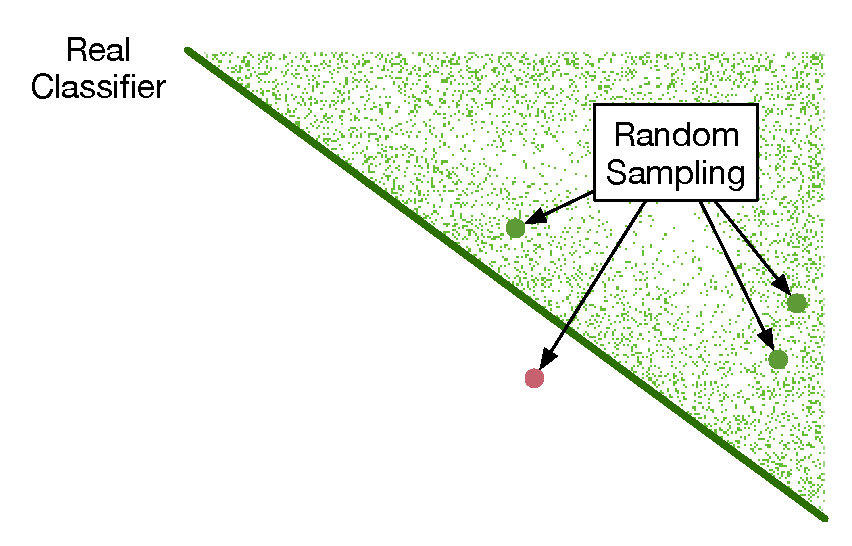
\includegraphics[scale=0.3]{figures/general-sampling-0.pdf}
        \caption{Random Sampling}
        \label{fig:sampling:random}
    \end{subfigure}
    \begin{subfigure}{0.23\textwidth}
        \centering
        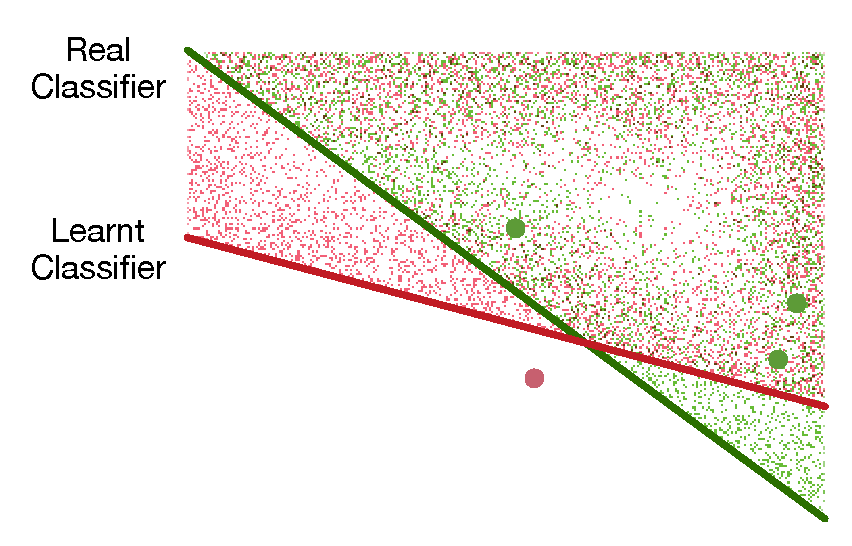
\includegraphics[scale=0.3]{figures/general-sampling-1.pdf}
        \caption{Learnt Invariant}
        \label{fig:sampling:random:invariant}
    \end{subfigure}
    \begin{subfigure}{0.23\textwidth}
        \centering
        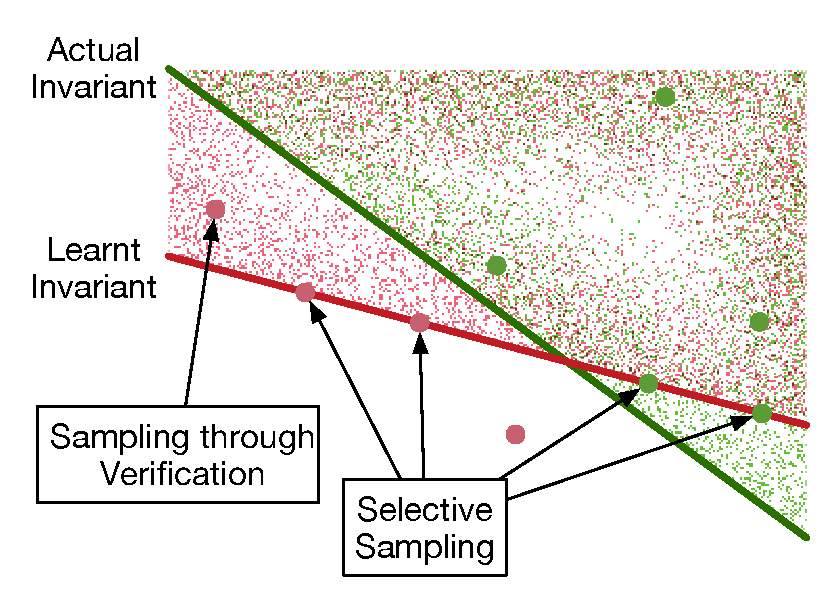
\includegraphics[scale=0.3]{figures/general-sampling-2.pdf}
        \caption{Selective and Counter-Example Sampling}
        \label{fig:sampling:selective}
    \end{subfigure}
    \begin{subfigure}{0.23\textwidth}
        \centering
        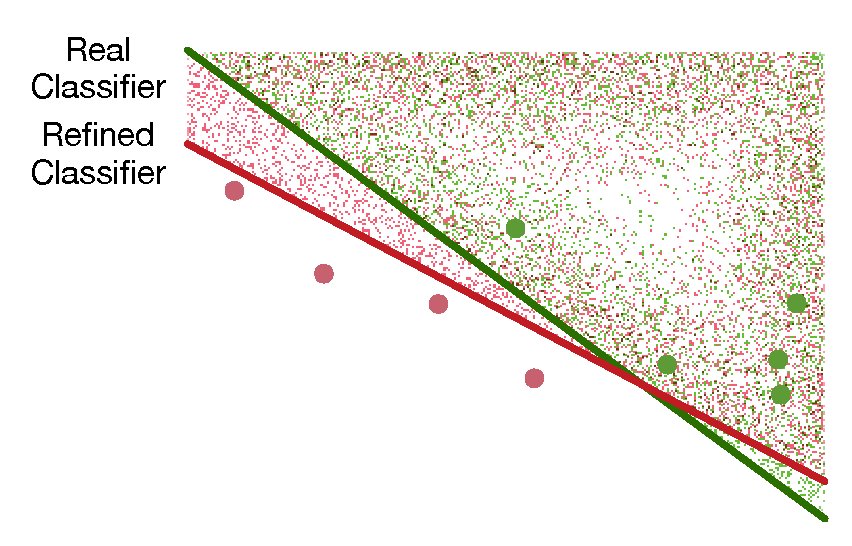
\includegraphics[scale=0.3]{figures/general-sampling-3.pdf}
        \caption{Refined Invariant}
        \label{fig:sampling:selective:invariant}
    \end{subfigure}
    \caption{Sampling Approaches}
    \label{fig:sampling}
\end{figure}

\medskip\noindent
\textbf{Random Sampling.}
This technique produce samples with the uniform distribution over a given range $\mathcal{R}$.
It acts as an initialization sampling method 
as well as a supplementary sampling method in our framework. 
Firstly, before any classifier is learnt in our framework, 
we adopt simple random sampling solely to learn the initial candidate, 
which can be refined later in the invariant inference process. 
Secondly, the efficiency of other sampling methods, introduced in the following, 
depends largely on the similarity of the invariant candidate and the actual invariant. 
However, if the invariant candidate is very different from the correct invariant, 
random sampling can make the candidate converge faster than other sampling methods. 
Thirdly, since selective sampling can introduce biased samples distribution, 
random sampling aims at reducing its impact that can lead to a biased candidate result. 
As a result, the random sampling, as an important sampling approach, 
is applied to all the invariant inference iterations. 

\medskip\noindent
\textbf{Selective Sampling.}
%Selective sampling is adopted in our framework to actively generate the samples 
%on the borders of the learnt invariant candidate. 
%These samples are very informative and instructive for invariant refinement, 
%as they give clear instructions on the amendment of the candidate.
Due to the limited number of samples we can gather in reality, 
we prefer the technique which generates samples that can vary the classifier than which does not.
%the invariant candidate obtained from these data might be far from being correct. 
%\LL{I think selective sampling is worse than random sampling 
%if the invariant is very different from the correct one. }
%As we can not gather all the program states for learning in reality,
The concept of active learning or selective sampling refers to the approaches 
that aim at reducing the labeling effort by selecting only the most informative samples to be labeled.
Given a classifier, this approach selects the samples that are the closest to the classification boundary 
so that they are the most difficult to classify and the most informative to label,
thus they can give clear instructions on the amendment of the candidate.
For instance, SVM(supported vector machines) selective sampling techniques have been proven effective in achieving a high accuracy 
with fewer examples in many applications~\cite{DBLP:conf/mm/TongC01,DBLP:journals/jmlr/TongK01}. 
Since an SVM classification function is represented by support vectors which are the samples closest to the boundary, 
this selective sampling effectively learns an accurate function with fewer labeled data~\cite{DBLP:conf/icml/SchohnC00}.

%When we have a guess of loop invariants, we can apply selective sampling approach to finding more useful samples.
%Actually we apply this sampling method all along the learning procedure except the first iteration.
%\LL{I suggest do not use words like `obvious', nothing is obvious in a paper.}

%In fact, without labeled samples which are right on the boundary of the actual classifier, 
%it is very unlikely that we would find it. 
%Intuitively and intelligently, in order to get the `actual' classifier, 
%we would require samples which would distinguish the actual one from any nearby one, 
%This problem has been discussed and addressed in machine learning using active learning and selective sampling~\cite{DBLP:conf/icml/SchohnC00}.

 

%In our setting, this means that we should sample a program state right by the classifier and test the program 
%with that state to label that feature vector so that the classifier would be improved.


%Algorithm~\ref{alg:active} presents details on how active learning is implemented in \textsc{Zilu}. 
%At line 2, we obtain a classifier based on Algorithm~\ref{classify}. 
%We compare the newly obtained classifier with the previous one at line 4, if they are identical, we return the classifier; 
%otherwise we apply selective sampling so that we can generate additional labeled samples for improving the classifier. 
%In particular, at line 5, we apply standard techniques~\cite{DBLP:conf/icml/SchohnC00} to select the most informative sample. 
%Notice that in our setting, the most informative samples are those which are exactly on the lines and 
%therefore can be obtained by solving an equation system. 
%At line 8, we test the program with the newly generated samples so as to label them accordingly.
%After the above discussion, apparently the pre-requirement of selective sampling is there is a guess.
%In our setting, %after learning an candidate, 
%which is usually a single polynomials or conjunction or \LL{disjunction?} of polynomials,
As the solutions to boundary equation are the points lying on the boundary. 
we do selective sampling by solving the equation system using \textbf{GSL}~\cite{gough2009gnu} in our setting.
For example, if we get a candidate $\mathcal{C} = \{11-2*x^2+2*y>=0\}$,
we do selective sampling in the following steps:
\begin{itemize}
\item[1)] Randomly choose the variable in the classifier. Here we take $x$ as picked variable.
\item[2)] Generates values for any other variables based on uniform distribution over the range $\mathcal{R}$. For example, we assign $y$ to $12$.
\item[3)] Solve the boundary equation after substituting the variables with their values. If there is no solution, go back to 1). For our example, we can get $x = \sqrt{35}/2 = 2.9580$.
\item[4)] Add a random variance $\epsilon \in [-1, 1]$ to the value of the picked variable. Here we add $\epsilon = 0.4$ to the value of $x$, and thus the new value of $x$ is $3.3580$. 
\item[5)] Roundoff the values of all the variables to meet the type requirement in the given program. Here we have $\{(x,y) \mapsto (3, 12)\}$.
\end{itemize}

In step 4, we add a small variance to variables because sometimes the points just lies on the boundary are very hard to tell their labels. 
%\LL{this is however not clear how it is done.}
%As a result, this technique is applied all along the learning process except the very beginning.

\medskip\noindent
\textbf{Counter-Example Sampling.}
Counter-example sampling chooses samples lying in the difference zone between the invariant candidate and the actual invariant.
%Compared with the above sampling techniques, we should admit counter-example sampling is more directly and objective.  
In our framework, when a invariant candidate fails to be validated in the verification stage,
a counter-example, that can directly refute our invariant candidate, would be provided by constraint solvers.
We pick the counter-example as samples to feed the given program in the next learning iteration.
Therefore, this technique is only applied between two learning iterations.
%$\textsc{Zilu}$ tries to valid it using symbolic execution~\cite{king1976symbolic}\cite{khurshid2003generalized}
%(or known as concolic testing~\cite{sen2007concolic}) and constraint solving,
%which is shown in detail in Section ~\ref{sec:verification}.
%If it fails to validate, the constraint solver could provide us with counter-examples that can directly refute our invariant candidate.
%And as a result, it is quite useful for the invariant candidate refinement in the next learning procedure.

%\LL{This is oral language. 
%Meanwhile, I do not understand what you are trying to say here. }
%As counter-example sampling technique sounds good, it seems this technique should be applied almost all the time, 
%but the fact is it is applied only after failure of invariant candidate verification.
%That is because applying concolic testing and constraint solving is a more time-consuming job than the other two sampling methods.

% subsection sampling_approaches (end)

\subsection {Loop Execution}
With the samples $\mathcal{S}$ obtained above, 
we execute the program from the state $s$ in $\mathcal{S}$. 
From program execution, 
we can generate more program states and check their satisfiability to $Pre$ and $Post$.
%In this step,
%we execute the program from the initial state $s_0$, where $s_0 \in \mathcal{S}$ and $\mathcal{S}$ is obtained from the above technique.
We record the following information during one execution:
\begin{itemize}
\item $Trace\{s_0 \to s_1 \to ...\to s_i \to ... \to s_n\}$, 
where $s_0$ is the initial state before entering the loop, 
$s_i$ is the state just after executing loop $Body$ for $i$ times,
and $s_n$ is the state satisfying $\neg B$ and thus the execution jumps out the loop $Body$;
\item $s_0 \models Pre$ or $s_0 \models \neg Pre$;
\item $s_n \models Post$ or $s_n \models \neg Post$.
\end{itemize}
For example, if we start the program execution with the sample $\{(x,y) \mapsto (3, 12)\}$ from the last selective sampling,
we could record a trace $Trace\{s_0 \to s_1 \to s_2\}$ where 
$s_0=\{(x,y) \mapsto (3, 12)\}$, $s_1=\{(x,y) \mapsto (13, 15)$ and $s_2=\{(x,y) \mapsto (23, 18)\}$,
and $s_0 \models Pre$ and $s_2 \models Post$.


\subsection {Labeling}
%\LL{I feel the labeling and sampling described here are inaccurate.
%Sampling should include all of the samples rather than only the initial inputs. 
%We can discuss later. }
%With the samples $S$ obtained above, we execute the program with initial state $s$ in $S$. 
%\LL{Here, the initial state is unclear. what is program state. }
%From program execution, we can generate more program states and check their satisfiability to $Pre$ and $Post$.
%In this step, we present the technique how we label them according to these information. 

To demonstrate the technique, a few symbols should be introduced first. 
$Body(s)$, defined in Section~\ref{sec:introduction}, is the state which could be reached after executing $Body$ from state $s$.
$Body^*(s)$ denotes the set of program states which could be reached after executing zero or more iterations of the loop starting from $s$.
Furthermore, we write $s \multimap s'$ to denote that starting with a program state $s$ would result in state $s'$ when the loop terminates. 
%\LL{I suggest use $\rightarrow$, $\rightarrow^*$ and $\multimap$. }
%\LL{What is Trace, defined?}
So if there is an execution trace $Trace\{s_0 \to s_1 \to ...\to s_i \to ... \to s_n\}$, 
%where $s_0$ is the initial state before entering the loop, 
%$s_i$ is the state just after executing loop $Body$ for $i$ times,
%and $s_n$ is the state satisfying $\neg B$ and thus the execution jumps out the loop $Body$,
then we have
\begin{itemize}
\item $s_{i+1} = Body(s_i)~~~~\forall i \in [0, \ldots, n-1]$.
\item $s_{i} \in Body^*(s_0)~~~~~~\forall i \in [0, \ldots, n]$.
\item $s_{0} \multimap s_{n}$.
\end{itemize}
%We write $Body^*(S)$ to denote $\{s' | \exists s \in S \cdot s' \in Body^*(s)\}$. 

\medskip\noindent
\textbf{Positive State, Negative State and Implication Pair}
%defines the label to a state.
are three concepts are originally introduced in \cite{sharma2014invariant}.
They tell whether a state must satisfy the loop invariant or must not.
A positive state is a state that must satisfy the actual loop invariant,
while a negative state is a state that must not satisfy the invariant.
An implication pair is a pair of state, the latter one satisfying the invariant 
if the former one satisfies it. 
In this part, we demonstrate the rules to category a state according to its execution information.
%In this paper, we use predicates and sets of states interchangeably.
\LL{I feel you do not need to put them as a section (I mean that it should not look like above). 
Say the positive states and the positive trace together.}

%Let $\mathcal{C}$ be a candidate invariant.

From constraint~\ref{inv:pre} we know, for an invariant $Inv$, 
any state satisfying $Pre$ should also satisfies $Inv$. 
Therefore, the state satisfying $Pre$ must be a positive state. 
\LL{Why do you want to say that it must be a positive state?}

\LL{The following is extremely hard to understand (grammar error). 
Give definition first, purpose later.}
The adjacent states $(s, t)$ appeared in a trace a pair of states is an implication pair,
because, according to the inductive property~\ref{inv:loop},
$(s \models Inv) \Rightarrow (t \models {Inv})$
if $t = Body(s)$ and $s \models Cond$.
On the contrary, for an invariant candidate $\mathcal{C}$, 
if there is an implication $(s, t)$ in which $(s \models \mathcal{C}) \wedge (t \models \neg \mathcal{C})$,
$\mathcal{C}$ is proved to be an invalid invariant.

Finally, a state satisfying $\neg{Cond} \wedge \neg{Post}$ must be a negative state.
Considering constraint~\ref{inv:post}, if a state $s \models \neg{Post}$,
then $s \models \neg(Inv \wedge \neg Cond)$.
In this situation $s \models \neg Cond$, then we can infer $s \models \neg Inv$. 
%The `existence of a state $s \models \mathcal{C} \wedge \neg B \wedge \neg Post$ proves $\mathcal{C}$ is inadequate to discharge the postcondition. 
%We call a state $s$ which satisfies $\neg{B} \wedge \neg{Post}$ a negative state. 

\medskip\noindent
\textbf{Positive Trace, Negative Trace, Implication Trace.}
\LL{Change above, do not put them as a section title.}
As an execution trace contains more data than a single state,
this part discusses the technique to label all the states in one trace at a time rather than just a single state.
Similar to the state labeling, a positive trace defines a trace with all positive states,
while a negative trace defines a trace with all negative states.
An implication trace is a trace in which, if one state is the positive state, 
all the states afterwards are positive states.
We state the regulation to determine the class of any given trace as follows.

For a trace $Trace\{s_0 \to s_1 \to ... \to s_i \to ... \to s_n\}$, 
if $s_0 \models Pre$, and $s_n \models Post$,
then this is a positive trace, meaning $\forall s_i \models Inv$.
Because if state $s_0$ satisfy $Pre$,
$s_0$ is a positive state that must satisfy $Inv$. %, according to equation 1.
Considering constraint~\ref{inv:loop}, $s_1$ is also positive states.
Then all the states in $Trace\{s_0 \to s_1 \to ...\to s_i, ... \to s_n\}$ are positive states inductively. 
%So now we can get a positive trace  $Trace\{s_0 \to s_1 \to ...\to s_i \to ... \to s_n\}$.

On the contrary, for a trace $Trace\{s_0 \to s_1 \to ...\to s_i \to ... \to s_n\}$, 
if $s_0 \models \neg Pre$, and $s_n \models \neg Post$,
we can infer this is a negative trace in the similar way. 
%which means all the states in this trace should be negative states.  
\LL{Make these two as theorems. Also define all the notations first. }

%Actually for an arbitrary trace, there are also two other possibilities we have not mentioned yet.

The third case is a trace that begins with a state $s_0 \models Pre$ and ends with a state $s_n \models \neg Post$,
\LL{obviously}, this is a counter-example to disprove the program and its specification.
As a result, if $\textsc{Zilu}$ meets any counter-example trace in the testing, 
the execution exits immediately with a failure message indicating a bug in the program. 

The last case is a trace begin with a state $s_0 \models \neg Pre$ but ends with a state $s_n \models Post$.
Under this condition, we could not determine whether $s_0$ and $s_n$ satisfy invariants or not,
not to mention other states $\{s_1, s_2, ..., s_{n-1}\}$.
Then this trace belongs to the implication trace set, meaning if $s_i \models Inv$, then $s_j \models Inv$ $\forall j \ge i$.
Implication traces can not be used to learn classifiers directly, 
however, they have power in validating a candidate.
For instance, providing a candidate $\mathcal{C} = x - y \ge 0$ and an implication trace 
$Trace\{s_0 \to s_1 \to s_2\}$ where 
$$s_0 = \big(x \mapsto 2, y \mapsto 1\big),  s_1 = \big(x \mapsto 2, y \mapsto 2\big),  s_2 = \big(x \mapsto 2, y \mapsto 3\big),$$
we could refute this candidate instantly.
For using $\mathcal{C}$ to label this whole trace as $$s_0 \mapsto +,  s_1 \mapsto +,  s_2 \mapsto -,$$ 
we find this violates the above implication rules,
indicating the current candidate $\mathcal{C}$ must be not an actual invariant.
%In this case, $\textsc{Zilu}$ return to sampling stage to get more data for learning.
%In total, we can have table.~\ref{LabelingTable}.
\LL{The missing part here is how you used it in this work.}


In total , we can categorize all the program states $Body^*(S)$ started from Set $S$ into four sets according to the following table.
In the Table~\ref{tab:labeling}
$\mathcal{S}^\chi$ stands for counter-example trace;
$\mathcal{S}^+$ stands for positive traces;
$\mathcal{S}^-$ stands for negative traces; 
and $\mathcal{S}^\rightarrow$ stands for implication traces.

%They can be judged according to Table~\ref{tab:labeling}: 
\begin{table}[htb]
\label{tab:labeling}
\centering
\begin{tabular}[float]{|c|c|c|}
\hline
$s_0 \Rightarrow \Rightarrow s_n$ & $s_n \models Post$            & $s_n \models \neg Post$\\
\hline
$s_o \models Pre$                 & $Body^*(s_0) \in \mathcal{S}^+$       & $Body^*(s_0) \in \mathcal{S}^\chi$\\
\hline
$s_0 \models \neg Pre$            & $Body^*(s_0) \in \mathcal{S}^\rightarrow$       & $Body^*(s_0) \in \mathcal{S}^-$\\
\hline
\end{tabular}
\caption{Trace Labeling Table}
\end{table}

% section sampling (end)

%!TEX root = paper.tex

\section{Classification} % (fold)
\label{sec:classification}

After sampling and labeling in the last step, we obtain some program states must be in $Inv$ and some must not. 
Thinking as a data scientist, if we view these program states as a data set, 
the problem to find an invariant candidate becomes the problem to find a classifier to divide the dataset according to their labels.
Fortunately, We can borrow the idea from machine learning area as the community has studied this problem has been fully studied several years ago.
and senior machine learning experts have developed several efficient supervised classification algorithms to handle this problem.

Before coming to the specific technique $\textsc{Zilu}$ applies,
it should be noted that there are at least two main differences between traditional machine learning problems and the problem in our setting:
\begin{itemize}
\item Most machine learning techniques care more about prediction correctness rather than understanding the underlying problem,
although there is a research trend in machine learning to understand ongoing during these years.
On the contrary, in software engineering area, program verification cares about formalization and reasoning.
As a result, a classification technique would be highly suggested as long as it can predict correctly on newly received data.
But in our setting, we need an explicit classifier which is readable by human and can proceed by off-the-shelf constraints solvers.
\item Machine learning algorithms think more of generalization ability than correctness on the training data.
Sometimes they can sacrifice the prediction correctness on the training data to exchange for higher generalization ability.
But in our setting, the first thing we care about is the prediction  correctness on the training data,
meaning we can not tolerate any slight classification error on the training set.
On this basis, we hope the classification algorithm can have better generalization ability.
\end{itemize} 

Among plenty of classification approaches, $\textsc{Zilu}$ takes Supported Vector Machines as a primary approach.

\subsection{Supported Vector Machines}
%, is one of the most powerful approaches.
%SVM is a supervised learning model with associated learning algorithms that analyze data used for classification. 
%In most setting, given a set of training examples, each marked as belonging to one of two categories, 
%an SVM training algorithm builds a model, which is a representation of the examples as points in space,
%that can assign new examples into one category or the other, 
%making it a non-probabilistic binary linear classifier. 

Supported Vector Machines, known as $\textsc{Svm}$, is a supervised machine learning algorithm for classification and regression analysis. 
We use its binary classification functionality. 
Mathematically speaking, the binary classification functionality of (linear) $\textsc{Svm}$ works as follows. 
Given two sets of feature vectors $S^+$ and $S^-$, it generates, if there is any, 
a linear constraint in the form of $ax + by + \cdots \geq d$ where $x$ and $y$ are feature values and $a, b, d$ are constants, 
such that every state $s \in S^+$ satisfies the constraint and every state $s' \in S^-$ fails the constraint. 
In the following, we write $\textsc{Svm}(S^+, S^-)$ to denote the function which returns a linear classifier.

%SVM

As differences between machine learning problem and our setting are discussed in the above subsection, in order for our approach to work,
$\textsc{Zilu}$ tunes $\textsc{LibSvm}$ in the following three aspects: 
\begin{itemize}
\item $\textsc{Svm}$ technique does not really calculate a hyperplane explicitly, 
but emits some supported vectors (this is where $\textsc{Svm}$ get its name) and some parameters.
%This might not a big problem if we do not apply $\textsc{Svm}$ with some kernel method (which is used to classify no linear separable data).
However in verification, we need an explicit classifier which is readable by human and can be proceeded by off-the-shelf constraints solvers.
Thus, we need to convert the $\textsc{Svm}$ model to a hyperplane by ourselves.
(This is also the reason we do not apply $\textsc{Svm}$ with kernel methods,
as converting $\textsc{Svm}$ models with kernel methods, i.e. $\textsc{Rbf}$ kernel, would be too complicated, sometimes even impossible.)
\item As $\textsc{Zilu}$ thinks higher of the correctness on the training data than anything else,
Before applying $\textsc{Svm}$ technique, the parameters (mainly $C$ which tells the $\textsc{Svm}$ optimization how much you want to avoid misclassifying each training example)
%different from $\mathcal{C}$ used as loop invariant candidate in our context) 
should be tuned to get a classifier which does a better job of getting all the training points classified correctly.
\item What's more, we need to check the classification correctness of the learned classifier 
on $\mathcal{S}^+$ and $\mathcal{S}^-$ to ensure that is a perfect classifier.
And $\textsc{Zilu}$ also takes $\mathcal{S}^\rightarrow$ to check the classifier(as is shown in Section 2).
\end{itemize} 

So the whole classification algorithm is described in ~\ref{alg:classify}.

\begin{algorithm}[!h]
\SetAlgoVlined
\Indm
\KwIn{$\mathcal{S}^+$, $\mathcal{S}^-$, and $\mathcal{S}^\rightarrow$}
\KwOut{$\textsc{Null}$ or a perfect classifier for $\mathcal{S}^+$ and $\mathcal{S}^-$ without violating $\mathcal{S}^\rightarrow$}
\Indp
    let $f$ = $\textsc{Svm}$($\mathcal{S}^+$, $\mathcal{S}^-)$\;
    \If {$f$ violates any data in $\mathcal{S}^+$ or $\mathcal{S}^-$} {
        \Return $\textsc{Null}$\;
    }
    \If {$f$ violates any inference rules in $\mathcal{S}^\rightarrow$} {
        \Return $\textsc{Null}$\;
    }
    \Return $f$;
\caption{Algorithm $classify$}
\label{alg:classify}
\end{algorithm}

It is noted that customers can substitute $\textsc{Svm}$ with other classification techniques for learning invariant. 
We will show this in ``$\textsc{Svm}$ derivatives'' part in the end of this section.
 
%In the following, we present how we obtain a classifier automatically using $\textsc{Svm}$. 
%In this work, we always choose the \textit{optimal margin classifier} (see the definition in~\cite{Sharma2012}) if possible. 
%This half space could be seen as the strongest witness why the two data states are different. 
%In the following, we write $svm(S^+, S^-)$ to denote the function which returns a linear classifier

%\subsection{Checking}
%With the learned $\textsc{Svm}$ model,we check whether it can perfectly classify these states first.
%If yes, then we can automatically turn it back to a hyperplane form, which is regarded as our invariant candidate.
%Otherwise, we may apply other classification techniques for learning, which will be mentioned at ``$\textsc{Svm}$ derivatives'' part in the end of this section.


\subsection{Active Learning} 
Algorithm~\ref{alg:active} presents details on how active learning is implemented in \textsc{Zilu}. 
At line 2, we obtain a classifier based on Algorithm~\ref{classify}. 
We compare the newly obtained classifier with the previous one at line 4, if they are identical, we return the classifier; 
otherwise, we apply selective sampling so that we can generate additional labeled samples for improving the classifier. 
In particular, at line 5, we apply standard techniques~\cite{DBLP:conf/icml/SchohnC00} to select the most informative sample. 
Notice that in our setting, the most informative samples are those which are exactly on the lines and therefore can be obtained by solving an equation system. 
At line 8, we test the program with the newly generated samples so as to label them accordingly.
\begin{algorithm}[h]
\SetAlgoVlined
\Indm
\KwIn{$\mathcal{S}^+$, $\mathcal{S}^-$, and $\mathcal{S}^\rightarrow$}
\KwOut{an invariant candidate $\mathcal{C}$}
\Indp
let $old_f$ be $null$\;
\While{true} {
    let $f$ = classify($\mathcal{S}^+$, $\mathcal{S}^-$, $\mathcal{S}^\rightarrow$)\;
    \If {$f$ is not equal to $\textsc{Null}$} {
        \If {$f$ is identical to $old_f$} {
            $\mathcal{C}$ = $f$\;
            \Return $\mathcal{C}$;
        }
        let $old_f = f$\;
    }
  %\textsc{Re-sampling}:\\
    $sam$ = selectiveSampling($old_f$)\;
    test the target program with $sam$\;
    update $\mathcal{S}^+$, $\mathcal{S}^-$, and $\mathcal{S}^\rightarrow$ accordingly\;
}
\caption{Algorithm $activeLearning$}
\label{alg:active}
\end{algorithm}


\begin{example}
\LL{to be added}
\end{example}

\begin{proposition}
Algorithm $activeLearning$ always eventually terminates. \hfill \qed
\end{proposition}


\subsection{SVM Derivatives}
%$\mathcal{S}^+$, $\mathcal{S}^-$, and $\mathcal{S}^\rightarrow$
If $\mathcal{S}^+$, $\mathcal{S}^-$ cannot be perfectly classified by one half-space only, 
a more complicated function $f$ must be adopted. 
For instance, if there is a classifier in the form of conjunctive of multiple half spaces, 
the algorithm presented in~\cite{Sharma2012} can be used to identify such a classifier.

Also in algorithm~\ref{alg:classify}, we mentioned customers can substitute $\textsc{Svm}$ with other classification algorithms for learning.
$\textsc{Zilu}$ has implemented two of them with native $\textsc{Svm}$: 
$Polynomial \textsc{Svm}$, which can be used to learn invariants in the form of polynomials or the equivalent mixed conjunctive or disjunctives,
and $Conjunctive \textsc{Svm}$, which can learn invariants in the form of conjunctive of polynomials.

\subsubsection{Polynomial SVM}
In previous research, several papers ~\cite{**} have studied invariants with conjunctive form or disjunctive form.
However, there is still no efficient approach to learning these invariants.
In our research, we found sometimes convert the conjunctive or disjunctives to a polynomial expression might be a nice try to this problem.
For instance, if the target invariant 
$$\mathcal{C} = (x \ge x_0 \bigvee x \le x_1) \ where\ x_0 < x_1$$,
we can find a polynomial expression 
$$\mathcal{C}' = \big(x^2 - (x_0 + x_1)x + x_0x_1 \ge 0\big)$$ 
as an equivalent invariant.

Actually, polynomials are more powerful on this than they look at the first glance, especially univariate polynomials. 
Some cubic univariate polynomials can represent disjunctive of a conjunctive expression and a linear expression.
For example, the following two expressions are equivalent:
$$\big(x \ge x_0 \bigwedge x \le x_1) \bigvee x \ge x_2\big) \ where\ x_0 < x_1 < x_2$$
$$x^3 + (x_0x_1 + x_0x_2 + x_1x_2)x^2 - (x_0 + x_1 + x_2)x - x_0x_1x_2 >= 0$$ 


This leads us to develop a classification algorithm for learning polynomial divider.
In practice, we map raw data (program states) in $\mathcal{S}^+$, $\mathcal{S}^-$ and $\mathcal{S}^\rightarrow$ to data in high dimensions, 
and then apply $\textsc{Svm}$ on the mapped data to learn a polynomial classifier. 
For now, $\textsc{Zilu}$ provide polynomials up to degree 4 as we think degree 4 can cover most hackneyed invariants.

But for the multivariate invariant problem, multivariate polynomials can not handle in most cases.
For example, $\mathcal{C} = (x \ge 0 \bigwedge y \ge 0)$,
it can be proved that there is no such a polynomial which can be equivalent with it.
So $\textsc{Zilu}$ apply Conjunctive SVM to solve this case.

\subsubsection{Conjunctive SVM}
In order to learn invariants in form of conjunctives, 
Rahul Sharma and others have developed a algorithm called ``$\textsc{Svm\_i}$'' in ~\ref{sharma2012interpolants},
but they failed to simplify the learned classifier.
$\textsc{Zilu}$ applied a technique ~\ref{alg:conjunctiveSVM} based on their $\textsc{Svm\_i}$ algorithm:

\begin{algorithm}[!h]
\SetAlgoVlined
\Indm
\KwIn{$\mathcal{S}^+$, $\mathcal{S}^-$}
\KwOut{a set of perfect classifiers for $\mathcal{S}^+$ and $\mathcal{S}^-$}
\Indp
    let $\mathcal{C}$ = $\textsc{Null}$\;
    let $\textsc{Misclassified}$ = $\mathcal{S}^-$\;
    \While {$\textsc{Misclassified}$ is not empty} {
        Random choose $s$ from $\textsc{Misclassified}$\;
        let $f$ = $\textsc{Svm}$($\mathcal{S}^+$, s)\;
        add $f$ to $\mathcal{C}$\;
        \For {$s' \in \textsc{Misclassified}$} {\
            \If {$f(s') \le 0$} {
                remove $s'$ from $\textsc{Misclassified}$\;
            }
        }
    }
    \For {$c \in \mathcal{C}$} {
        \If {$\mathcal{C}\diagdown c \Rightarrow c$} {
            remove $c$ from $\mathcal{C}$\;
        }
    }
    \Return $\mathcal{C}$;
\caption{Algorithm $conjunctiveSVM$}
\label{alg:conjunctiveSVM}
\end{algorithm}



%\section{Active Learning}
%Due to the limited set of samples we have (which is often referred to as labeled samples in the machine learning community), 
%the guessed classifier obtained from the previous iteration might be far from being correct. 
%In fact, without labeled samples which are right on the boundary of the `actual' classifier, 
%it is very unlikely that we would find it. 
%Intuitively, in order to get the `actual' classifier, we would require samples which would distinguish the actual one from any nearby one. 
%This problem has been discussed and addressed in the machine learning community using active learning and selective sampling~\cite{DBLP:conf/icml/SchohnC00}.

%The concept of active learning or selective sampling refers to the approaches 
%that aim at reducing the labeling effort by selecting only the most informative samples to be labeled. 
%SVM selective sampling techniques have been proven effective in achieving a high accuracy 
%with fewer examples in many applications~\cite{DBLP:conf/mm/TongC01,DBLP:journals/jmlr/TongK01}. 
%The basic idea of selective sampling is that at each round, 
%we select the samples that are the closest to the classification boundary so that they are the most difficult to classify and the most informative to be labeled. 
%Since an SVM classification function is represented by support vectors which are the samples closest to the boundary, 
%this selective sampling effectively learns an accurate function with fewer labeled data~\cite{DBLP:conf/icml/SchohnC00}. 
%In our setting, this means that we should sample a program state right by the classifier and test the program 
%with that state to label that feature vector so that the classifier would be improved.


% section classification (end)
%!TEX root = paper.tex

\section{Selective Sampling}
Due to the limited set of samples we have (which is often referred to as labeled samples in the machine learning community), the classifier obtained above might be far from being correct. In fact, without labeled samples which are right on the boundary of the `actual' classifier, it is very unlikely that we would find it. Intuitively, in order to get the `actual' classifier, we would require samples which would distinguish the actual one from any nearby one. This problem has been discussed and addressed in the machine learning community using active learning and selective sampling~\cite{DBLP:conf/icml/SchohnC00}.

\begin{algorithm}[t]
\SetAlgoVlined
\Indm
\KwIn{$F^+$ and $F^-$}
\KwOut{a classifier for $F^+$ and $F^-$}
\Indp
let $old$ be $null$\;
\While{true} {
    let $f = classify(F^+, F^-)$\;
    \If {$f$ is identical to $old$} {
        \Return $f$;
    }
    let $old = f$\;
    let $sam$ be a set of samples computed by selective sampling\;
    test the program and update $F^+$ and $F^-$ accordingly\;
}
\caption{Algorithm $activeLearning$}
\label{alg:active}
\end{algorithm}

The concept of active learning or selective sampling refers to the approaches that aim at reducing the labeling effort by selecting only the most informative samples to be labeled. SVM selective sampling techniques have been proven effective in achieving a high accuracy with fewer examples in many applications~\cite{DBLP:conf/mm/TongC01,DBLP:journals/jmlr/TongK01}. The basic idea of  selective sampling is that at each round, we select the samples that are the closest to the classification boundary so that they are the most difficult to classify and the most informative to label. Since an SVM classification function is represented by support vectors which are the samples closest to the boundary, this selective sampling effectively learns an accurate function with fewer labeled data~\cite{DBLP:conf/icml/SchohnC00}. In our setting, this means that we should sample a program state right by the classifier and test the program with that state to label that feature vector so that the classifier would be improved.

Algorithm~\ref{alg:active} presents details on how active learning is implemented in \textsc{Zilu}. At line 2, we obtain a classifier based on Algorithm~\ref{classify}. We compare the newly obtained classifier with the previous one at line 4, if they are identical, we return the classifier; otherwise we apply selective sampling so that we can generate additional labeled samples for improving the classifier. In particular, at line 5, we apply standard techniques~\cite{DBLP:conf/icml/SchohnC00} to select the most informative sample. Notice that in our setting, the most informative samples are those which are exactly on the lines and therefore can be obtained by solving an equation system. At line 8, we test the program with the newly generated samples so as to label them accordingly.

\begin{algorithm}[t]
\SetAlgoVlined
\Indm
\KwIn{$Pre$, $Cond$, $Body$, $Post$}
\KwOut{an invariant which completes the proof or a counterexample}
\Indp
let $T$ be a set of random samples\;
\While{true} {
    test the program for each sample in $T$\;
    \If {a state $s$ in $CT$ is identified} {
        \Return $s$ as a counterexample;
    }
    let $P$, $N$ and $NP$ be the respective sets accordingly\;
    let $Inv_u = activeLearning(P, N \cup NP)$\;
    let $Inv_o = activeLearning(P \cup NP, N)$\;
    let $Inv_s = activeLearning(P, N)$\;
    \For {each $Inv$ in $\{Inv_u, Inv_o, Inv_s\}$} {
        \If {(1) or (2) or (3) is not satisfied} {
            add the counterexample into $T$\;
        }
        \Else {
            \Return $Inv$ as the proof;
        }
    }
}
\caption{Algorithm $overall$}
\label{alg:overall}
\end{algorithm}

\begin{example}
\end{example}

\begin{proposition}
Algorithm $activeLearning$ always eventually terminates. \hfill \qed
\end{proposition}

\section{Verification}
Given a learned predicate $Inv$, we verify whether constraint (1), (2) and (3) are satisfied using symbolic execution. If all of them are satisfied, we successfully verify the program. Otherwise, if any of them is violated, the counterexample obtained is added to the set of sample $X$, which is then tested, categorized, used for active learning accordingly. The overall algorithm is presented in Figure~\ref{alg:overall}.

We remark that we learn three classifiers as candidates for the loop invariant: $U$, $OU$, $O$ such that
\begin{itemize}
\item $U$ classifies states in $P$ and those in $N \cup NP$.
\item $O$ classifies states in $N$ and those in $P \cup NP$.
\item $OU$ classifies states in $P$ and $N$;
\end{itemize}
Intuitively, $U$ would be an under-approximation of $Inv$ (by assuming states in $NP$ does not satisfy $Inv$); $O$ would be an over-approximation of $Inv$ (by assuming states in $NP$ does satisfy $Inv$); and $OU$ would be an safe-approximation of $Inv$ (by using states which we are certain whether they are in $Inv$ or not).
\begin{example}
\end{example}


\begin{theorem}
Algorithm $overall$ always eventually terminates and it is correct. \hfill \qed
\end{theorem}

%!TEX root = paper.tex

\section{Evaluations} % (fold)
\label{sec:evaluations}
We have implemented our invariant inference framework in a tool, called \textsc{Zilu}. \textsc{Zilu} is written using a combination of C++ as well as shell codes (for invoking external tools).
\textsc{Zilu} makes use of GSL~\cite{gough2009gnu} to solve equation systems which is necessary for selective sampling and
%% uses
 LibSVM~\cite{chang2011libsvm} as a primitive classification engine for
SVM-based learning classifier. %% based on SVM.
For invariant verification, we %% reuse a large part of
adopt the KLEE project~\cite{cadar2008klee} to
symbolically execute
%% generate verification conditions for
 C programs %% and use
prior to invoke Z3~\cite{de2008z3} for checking satisfiability of
the formulas (4), (5) and (6).
 We remark that KLEE is a concolic symbolic executor; it may
concretely execute the programs and return 
 under-approximated
abstraction. This may affect the soundness of our system.
To overcome this problem, we detect those path conditions produced from
concrete executions
and return sound abstraction, i.e. $true$, for them.
 %% KLEE was designed for test case generation and thus its default encoding may result in under-approximation of the program behavior. We have re-implemented the relevant part of KLEE to make sure the right verification conditions are generated.

Our test subjects include a set of benchmark programs %% which we
(i) gathered from
 the previous publications on loop invariant generation~\cite{???}  as well as
 (ii)
%% benchmark programs
taken  from
 the software verification competition repository~\cite{Dirk:SVCOMP:2016}.
All benchmarks are available from~\cite{zilu}.
%% Note
We notice that loops of these benchmark programs often contain non-deterministic choices
%% in the loop
which are used to model I/O environment (e.g., an external function call).
As non-determinism is beyond the scope of this paper,
we syntactically replace these non-deterministic commands by  free boolean-type variables.
It would be interesting to investigate how
 our active learning verification system can be extended
to infer non-determinism-based invariants.
 %% which by our assumption is not allowed. We thus transform the programs so that free boolean-type variables are introduced to replace the non-deterministic choice. We remark that the assumption of no non-determinism is less a problem for verification programs in practice as they are often deterministic. These benchmark programs are made non-deterministic often as a way of abstracting away certain complicated (e.g., an external function call) part of the program which is irrelevant to proving/disproving the Hoare triple.
%In our experimental evaluation,
%we test \textsc{Zilu} with \LL{Number} loop invariant benchmarks
%in the following form, where $\mathit{Body}$ can have nested loops and conditional choices.
%\[
%   \{ \mathit{Pre} \} \mathit{while}(\mathit{Cond}) \{ \mathit{Body} \} \{ \mathit{Post} \}
%\]
%% Do not apply this to `add' more content to the paper.
%% It lefts lots of empty space which did the contrary thing.
%% \begin{align*}
%% &Pre&\\
%% &while (Cond) \{&\\
%% &  \quad Body &\\
%% &\} &\\
%% &Post &
%% \end{align*}
%\LL{Introduce the sources of the benchmark.}
 %% All benchmarks are available from~\cite{zilu}.

The parameters chosen in our experimental evaluation are as follows.
For random sampling, we generate random values of all input variables of the program from their default ranges. Be default, we generate XXX random samples. 
%which would be enlarged if we can not find samples in a few tries.
%Our experiments indicate this $\mathcal{R}$ is a relatively rational range for the initial sampling.
During classification, the parameter $C$ which is the preference between avoiding misclassifying each training example and enlarging decision boundary,
and the inner iteration for SVM learning are set to their maximum value so as to generate only perfect classifiers. Each invocation of the SVM classification engine is set to time out in XXX seconds. The maximum dimension for learning polynomial classifiers is set to be 3. For invariant verification, we encode integer-type variables in the programs as integers in Z3. 


%Considering the differences between machine learning problem and our setting,
%\textsc{Zilu} tunes $\textsc{LibSvm}$~\cite{chang2011libsvm} in the following three aspects in order to get a \underline{perfect classifier}.
%\begin{itemize}
%\item Convert \textsc{Svm} model to an explicit classifier.
%The original \textsc{Svm} technique does not explicitly calculate a hyperplane, but emits its own model
%which can be used to do prediction on the given data.
%%This might not a big problem if we do not apply $\textsc{Svm}$ with some kernel method (which is used to classify no linear separable data).
%However, we need a explicit classifier as the loop invariant candidate which can be understood and proceeded later for verification.
%(This is also why we do not apply $\textsc{Svm}$ with kernel methods~\cite{yu2009evolving},
%considering converting $\textsc{Svm}$ models with kernel methods, i.e. $\textsc{Rbf}$ kernel, would be a complicated, sometimes even impossible, task.)
%
%\item As \textsc{Zilu} treasures classification accuracy on the training dataset% than anything else,
%before applying primitive $\textsc{Svm}$ technique, the parameters
%(mainly $C$ which tells the $\textsc{Svm}$ optimization how much you want to avoid misclassifying each training example)
%%different from $\mathcal{C}$ used as loop invariant candidate in our context)
%should be carefully tuned to learn a perfect classifier which perform well on the training points.
%
%\item Validating the learned classifier.
%Checking the classification correctness of the learned classifier
%on $\mathcal{S}^+$ and $\mathcal{S}^-$ is still needed as our setting needs to ensure the learned classifier is a perfect one.
%\textsc{Zilu} also takes $\mathcal{S}^\rightarrow$ to validate the learned classifier(as is shown in Section~\ref{sec:sampling}).
%\end{itemize}

\begin{table}[t]
\scriptsize
\centering
\caption{Statistics on TLV abstracting the classes, where N.A. stands for not available}
%\begin{tabular}{l c | c c c c | c c c c | c c }
%\cline{3-10}
\begin{tabular}{l c | c c c c| c c c | c c }
\cline{3-9}
%& &\multicolumn{4}{|c|}{\textsc{Zilu} with Selective}&\multicolumn{4}{c|}{\textsc{Zilu} without Selective} & & \\
& &\multicolumn{4}{|c|}{\textsc{Zilu} with Selective}&\multicolumn{3}{c|}{\textsc{Zilu} without Selective} & & \\
\hline
%\multicolumn{1}{|c|}{benchmark}&\multicolumn{1}{|c|}{inv type}& $\sharp$r. sample & $\sharp$s. sample & $\sharp$v. sample & time & $\sharp$r. sample & & $\sharp$v. sample & time & \multicolumn{1}{|c|}{Interproc} & \multicolumn{1}{|c|}{CPAChecker} \\
\multicolumn{1}{|c|}{benchmark}&\multicolumn{1}{|c|}{inv type}& $\sharp$r. samples & $\sharp$s. samples & $\sharp$v. samples &time(s) & $\sharp$r. samples & $\sharp$v. samples &time(s) & \multicolumn{1}{|c|}{Interproc} & \multicolumn{1}{|c|}{CPAChecker} \\
\hline % inserts single horizontal line
\multicolumn{1}{|c|}{afnp2014\_true\text{-}unreach\text{-}call}         	&conjunctive	&1056 &4224 & &259.38	&5160 & &295.03  & &  \\
\multicolumn{1}{|c|}{cav12foo1}         									&conjunctive 	&228 &912 &20 &51.07	&1980 &48 &168.97  & &  \\
\multicolumn{1}{|c|}{cav12foo2}         									&conjunctive 	&36 &144 &2 &16.09		&260 &6 &15.98  & &  \\
\multicolumn{1}{|c|}{cggmp2005\_variant\_true\text{-}unreach\text{-}call}   &conjunctive 	&210 &840 & &74045	&2220 & &timeout  & &  \\
\multicolumn{1}{|c|}{conj}         											&polynomial 	&10 &40 &2 &20.48		&70 &1 &28.48  & &  \\
%\multicolumn{1}{|c|}{conj}         											&conjunctive/polynomial & & &  &   &  & & &  & &  \\
\multicolumn{1}{|c|}{css2003\_true\text{-}unreach\text{-}call}         		&conjunctive 	&140 &560 & &36.02	&1220 & &83.29  & &  \\
\multicolumn{1}{|c|}{dis}         											&polynomial 	& & & &  &   & &  & &  \\
\multicolumn{1}{|c|}{down\_true\text{-}unreach\text{-}call\_1}         		&conjunctive 	&114 &256 & &116.21  &2160  &  &timeout  & &  \\
\multicolumn{1}{|c|}{down\_true\text{-}unreach\text{-}call\_2}         		&conjunctive 	&132 &528 & &27.5  &360 &   &timeout  & &  \\
\multicolumn{1}{|c|}{f2}         											&linear 		&52 &208 &1 &10.15  &120 &1   &12.03  & &  \\
\multicolumn{1}{|c|}{f3}         											&linear 		&36 &144 &1 &105.15  &330  &5  &93.04  & &  \\
%\multicolumn{1}{|c|}{fig1a\_1}         										&linear & & &  &   &  & & &  & &  \\
%\multicolumn{1}{|c|}{fig1a\_2}         										&linear & & &  &   &  & & &  & &  \\
\multicolumn{1}{|c|}{interproc\_test1}         								&linear 		&8 &32 &1 &9.21  &40 &2   &10.38  & &  \\
\multicolumn{1}{|c|}{interproc\_test2}         								&linear 		&84 &96 &1 &11.66  &240  &1  &171.14  & &  \\
\multicolumn{1}{|c|}{interproc\_test3}         								&linear 		&42 &168 &1 &30.32  &420 &5   &43.34  & &  \\
\multicolumn{1}{|c|}{interproc\_test4}         								&linear 		&28 &112 &4 &14.8  &240 &5   &38.25  & &  \\
\multicolumn{1}{|c|}{interproc\_test5}         								&linear 		&32 &128 &1 &9.18  &180 &3   &28.05  & &  \\
\multicolumn{1}{|c|}{interproc\_test6}         								&polynomial 	&6 &24 &1 &11.83  &70  &2  &18.27  & &  \\
\multicolumn{1}{|c|}{interproc\_test8}         								&conjunctive 	&24 &96 &6 &22.13  &220  &2  &97.47  & &  \\
\multicolumn{1}{|c|}{interproc\_test11}         							&linear 		&24 &96 &2 &24.79  &180 &2   &206.07  & &  \\
\multicolumn{1}{|c|}{lili2}         										&linear 		&84 &336 &4 &21.28  &720  &9  &82.24  & &  \\
\multicolumn{1}{|c|}{linear6}         										&linear 		&18 &72 &1 &16.19  &270 &3  &179.39  & &  \\
\multicolumn{1}{|c|}{multivar\_true\text{-}unreach\text{-}call1}         	&conjunctive 	&68 &272 &3 &16.84  &220 &4   &15.22  & &  \\
\multicolumn{1}{|c|}{terminator\_01\_safe}         							&linear 		&6 &24 &1 &9.2  &90  &4  &13.06  & &  \\
\multicolumn{1}{|c|}{test}         											&linear 		&28 &112 &1 &10.19  &420 &2  &24.51  & &  \\
\multicolumn{1}{|c|}{test2}         										&conjunctive 	&44 &176 &3 &79.45  &120  &3  &timeout  & &  \\
%\multicolumn{1}{|c|}{up\_true\text{-}unreach\text{-}call\_1}         		&conjunctive & & &  &   &  & & &  & &  \\
\multicolumn{1}{|c|}{up\_true\text{-}unreach\text{-}call\_2}         		&conjunctive 	&240 &960 &14 &84.02  &540 &7   &89.77  & &  \\
%\multicolumn{1}{|c|}{xeq10}         										&linear & & &  &   &  & & &  & &  \\
\multicolumn{1}{|c|}{xle10}         										&linear 		&6 &24 &1 &8.57  &60 &3   &12.58  & &  \\
\multicolumn{1}{|c|}{xy10}         											&linear 		&162 &648 &4 &39.69  &840  &11  &40.51  & &  \\
\multicolumn{1}{|c|}{xyle0}         										&polynomial 	& & & &  &   & &  & &  \\
\hline
\end{tabular}
\label{tbl:stats}
\end{table}

%\begin{table*}[t]
%    \begin{center}
%    % \begin{minipage}{\textwidth}
%    % \begin{adjustwidth}{-1in}{-1in}
%    \begin{center}
%    \begin{adjustbox}{max width=1\textwidth}
%    \begin{tabular}{l | r | r | r | r | r | r | r | r | r}
%        \hline\hline
%        Benchmark
%            & $\sharp$Random Samples & $\sharp$Selective Samples & $\sharp$Iterations
%            & $\sharp$Traces & $\sharp$Variables
%            & Time & Invariant Type
%            & Interproc & CPAChecker
%            \\
%        \hline
%        Linear 1
%            & 196 & 4 & 1
%            & 1 & 1
%            & 3.31s & Linear
%            & 0.01s & 3.42s
%            \\
%        \hline
%        Linear 2
%            & 3158 & 7 & 1
%            & 1 & 2
%            & 9.86s & Linear
%            & 0.01s & 3.29s
%            \\
%        \hline
%        Linear 3
%            & 11102 & 6 & 1
%            & 1 & 3
%            & 40.24s & Linear
%            & 0.01s & 3.50s
%            \\
%        \hline
%        Linear 4
%            & 1143 & 10 & 1
%            & 9 & 2
%            & 12.54s & Linear
%            & 0.01s & 3.76s
%            \\
%        \hline
%        Linear 5
%            & 918 & 8 & 2
%            & 3 & 2
%            & 14.47s & Linear
%            & Error & 3.66s
%            \\
%        \hline
%        Poly 1
%            & 64 & 7 & 2
%            & 1 & 1
%            & 10.51s & Polynomial
%            & Unknown & Unknown
%            \\
%        \hline
%        Poly 2
%            & 32711 & 85 & 7
%            & 2 & 2
%            & 23m43.1s & Polynomial
%            & Unknown & Unknown
%            \\
%        \hline
%        Poly 3
%            & 272 & 17 & 4
%            & 3 & 1
%            & 15.82s & Polynomial
%            & 0.01s & 3.31s
%            \\
%        \hline
%        Poly 4
%            & 2287 & 112 & 9
%            & 2 & 2
%            & 13m43.7s & Polynomial
%            & Unknown & Unknown
%            \\
%        \hline
%        Conjunction 1
%            & 21247 & 81 & 1
%            & 3 & 2
%            & 20m41.35s & Conjunction
%            & 0.01s & 3.16s
%            \\
%        \hline
%    \end{tabular}
%    \end{adjustbox}
%    \end{center}
%    % \end{adjustwidth}
%    % \end{minipage}
%    \end{center}
%    \caption{Experiment Results}
%    \label{tab:experiments}
%\end{table*}

We compared \textsc{Zilu} with two state-of-the-art invariant inference tools: Interproc~\cite{jeannet2010interproc} and CPAChecker~\cite{beyer2011cpachecker}. We remark many other tools have been reported~\cite{}, most of which are not maintained any more. The comparison between \textsc{Zilu} and Interproc or CPAChecker should be taken with a grain of salt as the methods for invariant generation are very different. Interproc is based on abstract interpretation. In the experiment, Interproc uses its most expressive abstract domain, i.e., the reduced product of polyhedra and linear congruences abstraction. Similar to \textsc{Zilu}, Interproc explicitly labels the loop invariants in the loop program. We thus can manually check their correctness and compare them with the invariants generated by \textsc{Zilu}. On the other hand, CPAChecker (formerly BLAST~\cite{henzinger2003software}) is a software verification tool based on the framework of configurable program analysis~\cite{beyer2007configurable}. In the experiment, CPAChecker is configured to generate loop invariants to prove the same Hoare triple. In addition, we compare the performance of \textsc{Zilu} with or without active learning in order to show the relevance of active learning and selective sampling.

The experiment results are presented in Table~\ref{tbl:stats}. All of the experiments are conducted using x86\_64 Ubuntu 14.04 (kernel 3.13.0-85-generic) with 2.3 GHz Intel Core i5 and 4G 1333MHz DDR3.
The first column shows which a name of the benchmark program. The second shows the type of invariant required for proving the Hoare triple. The next four columns present details on \textsc{Zilu}, i.e., the number random samples, selective samples, samples through verification and the execution time. The next four present the corresponding statistics running \textsc{Zilu} without selective sampling. The last two columns show the execution time of the two comparing tools.  
%%\LL{I need more information on the percentage of the samples. }
%`$\sharp$Invariants' stands the numbers of invariants generated by SVM,
%and `$\sharp$Iterations' represents the number of invariant candidates.
%Notice that an invariant generated by SVM becomes an invariant candidate
%when it converges to two previously generated invariants from SVM in one iteration process.
%`$\sharp$Traces' represents the number of loop body traces produced by KLEE~\cite{cadar2008klee}.
%and `$\sharp$Variables' represents the number of program variables.
% In general, when numbers of traces and variables increase in a program,
% the invariant inference difficulty increases.
%The seventh column gives the time used for the invariant generation
%and the eighth column gives the invariant type of the generated invariant.
We remark that since \textsc{Zilu} relies on generating random numbers, all numbers collected from \textsc{Zilu} in the table are the average of 10 experiments.

As can be seen from Table~\ref{tab:experiments},
some of the experiments take much longer time comparing with others,
with high numbers of samples, invariants, iterations.
The reason behind this is
that some variables are missing in the constraints of the loop invariant,
e.g., `Poly 2', `Poly 4' and `Conjunction 1'.
For instance, in the `Poly 1' case, the loop invariant is `$x^2 \le y^2$'.
However, the general form of a 2-order polynomial with 2 variables
is written as
\[
    a \cdot x^2 + b \cdot y^2 + c \cdot x y + d \cdot x + e \cdot y + f \le 0.
\]
Hence, we need to infer $c = d = e = f = 0$
which causes the difficulty of invariant inference.

The last two columns show the analysis results from Interproc and CPAChecker.
As can be seen, Interproc is extremely fast.
However, the invariant given by Interproc can be incorrect,
which can be demonstrated by the running example
that we introduced in Section~\ref{sec:introduction}.
In the running example, since we have $x < y$ constrained by the while loop condition,
it is thus impossible to execute the trace where $(x \ge 0) \land (y < 0)$.
However, Interproc outputs the loop invariant corresponding to this execution trace,
because the invariants in Interproc are global constraints
without considering their generation paths and conditions.
Both of Interproc and CPAChecker are faster than our tool \textsc{Zilu}.
On the other hand, \textsc{Zilu} can automatically generate polynomial loop invariants
which cannot be handled by Interproc and CPAChecker.

% section evaluations (end)

%!TEX root = paper.tex

\section{Conclusion and Related Work} % (fold)
\label{sec:related}
In this work, we propose an approach to improve loop invariant generation through guess-and-check. In particular, we propose to apply active learning techniques so as to learn accurate candidate loop invariants prior to the invariant checking phase. Furthermore, we propose a path-sensitive way of learning disjunctive loop invariants through classification. In principle, our approach can be extended to learn arbitrary mathematical classifiers using methods like SVM with kernel methods~\cite{svm:kernel}.
Nonetheless, due to the limited verification capability of existing program verification techniques, we focus on invariants in the form of polynomial inequalities or conjunctions/disjunctions of polynomial inequalities in our evaluation.
%Furthermore, we assume there is a bound $k$ on the number of clauses in the variant.
%In practice, we would expect (refer to empirical evidence in Section~\ref{sec:evaluations}) often $k$ is of a small value.


% \begin{table}
%     \begin{center}
%     \begin{tabular}{| l | c | c | l |}
%         \hline
%         Name & Inference Strategy & Inference Source \\
%         \hline
%         ABS & Eager & \\
%         \hline
%         CONS & Eager & \\
%         \hline
%         CEGAR & Lazy & Counterexample \\
%         \hline
%         INTER & Lazy & Counterexample \\
%         \hline
%         G\&C & Eager & Empirical \\
%         \hline
%         ABD & Lazy & Semantic \\
%         \hline
%         DAL & Eager & All Above \\
%         \hline
%     \end{tabular}
%     \end{center}
%     \caption{Existing Invariant Inference Approaches}
%     \label{tab:related}
% \end{table}

This work is closely related and inspired by the guess-and-check approach for loop invariant generation, documented in~\cite{sharma2012interpolants,sharma2013verification,DBLP:conf/esop/0001GHALN13,sharma2014invariant}.
In~\cite{sharma2012interpolants}, the authors proposed to learn loop invariants based on SVM classification.
The samples are generated through constraint solving. In~\cite{sharma2013verification}, the authors proposed to apply PAC learning.
It has been demonstrated that their approach may learn invariants in the form of arbitrary boolean
combinations of polynomial inequalities under certain assumptions. In~\cite{DBLP:conf/esop/0001GHALN13},
the authors developed a guess-and-check algorithm for generating algebraic equation invariants.
In~\cite{sharma2014invariant}, the authors proposed a framework for generating invariant based on randomized search.
In particular, their approach has two phases. The search phase uses randomized search to discover candidate invariants and the validate phase uses the checker to either prove or refute the candidate.
\textsc{Zilu} complements the above approaches with active learning so as to reduce the need of checking, sometimes completely. Furthermore, \textsc{Zilu} supports a new way of learning disjunctive invariants

In addition, this work is related to a large body of approaches on loop invariant generation. The existing approaches can be mainly categorized as:
the ones based abstract interpretation~\cite{cousot1978automatic,mine2006octagon,karr1976affine,vincent2009subpolyhedra}, %%,cousot1979systematic
the ones based on constraint synthesis~\cite{ashutosh2009invgen,michael2003linear,sumit2009constraint},
the ones based on counterexample-guided abstraction refinement ($\mathit{CEGAR}$)~\cite{henzinger2003software,thomas2001slam,edmund2003counterexample},
the ones based on computing interpolation~\cite{kenneth2010lazy,thomas2004abstractions,kenneth2003interpolation,Kenneth2006lazy},
the ones based on abductive inference~\cite{isil2013inductive},
the ones based on guess-and-check~\cite{cormac2001houdini,ernst2007daikon}.

On one hand, invariant inference methods based on abstract interpretation and constraint synthesis
often try to generate all possible invariants in certain domain~\cite{mine2006octagon,vincent2009subpolyhedra,ashutosh2009invgen},
regardless of whether they are useful to prove the Hoare triple or not.
As a result, the invariants inferred by them can be complex sometimes and yet fail to prove the program correctness.
On the other hand, other methods based on $\mathit{CEGAR}$, interpolation and abduction only generate those related to the program verification~\cite{isil2013inductive}.
Different from the above approaches, \textsc{Zilu} initially treats the given program as a black box and only collects relevant program states by executing the program.
This step has no scalability issue.
\textsc{Zilu} only opens up the black box after candidate invariants have converged.
From this point of view, \textsc{Zilu} is lightweight compared to the above approaches.
%In addition, \textsc{Zilu} adopts an active learning approach in an iterative refinement scheme.
%After generating the invariant, we check its correctness and refine it
%based on various new information (e.g., counter-examples, new samples)
%if it cannot prove the program correctness.
%Different from most of the existing refinement approaches,
%our method is driven by data samples
%rather than syntactic~\cite{cormac2001houdini} or semantic~\cite{ashutosh2009invgen,isil2013inductive} clues.
%Hence, it is more flexible and extensible to capture new types of invariants,
%and it is platform- and language-independent.
%Based on the needs in practice, under-approximation or over-approximation
%can also be applied to the data samples with ease.

% section related (end)

%!TEX root = paper.tex

\section{Conclusion} \label{conclusion}


\paragraph{Limitation and Potential Remedies}
We remark that in theory, we could learn arbitrary mathematical classifier using methods like SVM with kernel methods\cite{yu2009evolving}. 
Nonetheless, due to the limitation of proving capability and tools with regards to non-linear constraints, we leave those to our future work. 
Furthermore, we assume there is a bound $k$ on the number of clauses in the variant. 
In practice, we would expect (refer to empirical evidence in Section~\ref{sec:evaluations}) often $k$ is of a small value.


\bibliographystyle{abbrv}
\bibliography{learning}

\end{document}
